\documentclass[11pt,twoside]{article}
\usepackage{silence} % Filtert die harmlosen Font-Shape-Warnungen der hyphenat[htt]-Option
\WarningFilter{latexfont}{Font shape}
\WarningFilter{latexfont}{Some font shapes were not available}
\WarningsOff[hyphenat]
\usepackage[table]{xcolor} % Für farbige Tabellen
\usepackage[ngerman]{babel} % Für Silbentrennung und deutsche Spracheinstellungen
\usepackage[utf8]{inputenc} % Um Umlaute und Sonderzeichen nutzen zu können
\usepackage[T1]{fontenc} % Um Umlaute und Sonderzeichen nutzen zu können
\usepackage[scaled]{helvet}
\renewcommand{\familydefault}{\sfdefault}
\usepackage[a4paper,
	lmargin={2cm},
	rmargin={2cm},
	tmargin={2cm},
	bmargin={3cm}]{geometry} % Für das Layout und die Seitenränder
\usepackage{setspace} % Für den Zeilenabstand
\setstretch{1.15} % Zeilenabstand auf 1.5 setzen
\usepackage[skip=1pt plus 1pt minus 1pt]{parskip}
\raggedbottom
\usepackage{graphicx} % Um Bilder einzufügen
\usepackage{wrapfig} % Um Bilder im Fließtext einzubinden
\usepackage{csquotes} % Um Text in Anführungsstriche zu setzen
\usepackage{pdfpages} % Um die Titelseite und andere PDF-Seiten einzubinden
\usepackage{hyperref} % Um Verlinkungen und Hyperlinks einzufügen
\usepackage{acronym} % Um Akronyme zu definieren und zu verwalten
\usepackage{subcaption} % Um mehrere Bilder zusammen einzustellen und Links zu Abbildungen zu korrigieren
% Bildunterschriften einheitlich: 11pt, Label aufrecht, Text kursiv, Doppelpunkt.
% caption 3.6 kennt den Schluessel fontsize noch nicht -> eigene Schriftgroesse deklarieren.
\DeclareCaptionFont{beschriftung}{\fontsize{11pt}{13.2pt}\selectfont}
\captionsetup{font=beschriftung, labelfont=up, textfont=it, labelsep=colon}
\usepackage{dirtytalk} % Für Zitate: \say{...} zur einfachen Handhabung von Zitaten
\usepackage{textcomp} % Für Copyright, Trademark etc
\newcommand{\todo}[1]{ % TODO-Notizen erstellen
	\textcolor{red}{TODO: #1}
}
\newcommand{\note}[1]{\textcolor{blue}{NOTE: #1}
}
\usepackage{amsmath} % Für \text, Matheumgebungen
\usepackage{booktabs} % Für schönere Tabellen
\usepackage{tabularx}
\usepackage{listings}
\usepackage{enumitem}
\newcommand{\needCite}[1][]{
	\colorbox{yellow}{\textcolor{red}{Zitation Notwendig #1}}%
}

\newcommand{\anf}[1]{\glqq #1\grqq{}} % Anführungszeichen für Zitate
\usepackage{pdflscape}
\usepackage{longtable}
\usepackage{multirow}
\usepackage{array}
\usepackage{placeins}
\usepackage[htt]{hyphenat}   % erlaubt Umbrüche in \texttt

\usepackage[export]{adjustbox}
\usepackage{caption}

\usepackage{color,soul}
% Auskommentieren für APA
% (Zeile 125 auch auskommentieren)
%\usepackage{apacite}
%\bibliographystyle{apacite} % Zitierstil in APA

% Auskommentieren für IEEE
% (Zeile 128 auch auskommentieren)
\usepackage[style=apa, backend=biber]{biblatex} % Verwende biblatex für Zitationen im IEEE-Stil
\addbibresource{literature.bib} % Quellenverzeichnis einfügen
\DefineBibliographyStrings{ngerman}{%
  andothers = {et\addabbrvspace al\adddot}, % Anpassung für "et al." in der Literatur
}
% Umbruch für URLs in der Literatur
\usepackage{url} % Für die korrekte Darstellung von URLs
\setcounter{biburllcpenalty}{7000} % Strenge Umbruchregeln für URLs
\setcounter{biburlucpenalty}{8000} % Strenge Umbruchregeln für URLs

\setlength{\parindent}{0pt} % Einrücken bei Absatz verhindern

% \paragraph-Überschriften: Abstand davor wie bei einem normalen Absatz.
% Die Artikel-Klasse setzt hier standardmäßig 3.25ex, was neben dem
% parskip-Abstand von 1pt als Lücke auffällt.
% Mehr Luft gewünscht? Den ersten Wert unten auf z.B. 1ex erhöhen.
\makeatletter
\renewcommand\paragraph{\@startsection{paragraph}{4}{\z@}%
	{1pt \@plus 1pt \@minus 1pt}% Abstand davor
	{-1em}% Überschrift läuft in den Text (wie bisher)
	{\normalfont\normalsize\bfseries}}
\makeatother

\RequirePackage{fancyhdr} % Für benutzerdefinierte Kopf- und Fußzeilen

\cfoot{\thepage} % Seitenzahl in der Mitte des Fußbereichs

\newcounter{romanBeginningEnd} % Um Römische Seitenzahl zu speichern

% Sektionen Referenzen anpassen
\addto\extrasngerman{%
	\renewcommand{\sectionautorefname}{Kapitel}
	\renewcommand{\subsectionautorefname}{Abschnitt}
	\renewcommand{\subsubsectionautorefname}{Abschnitt}
}


\begin{document}


	\pagenumbering{gobble} % Seitenzahlen unterdrücken
	\newpage
\thispagestyle{empty}

\begin{center}
    \noindent

    \begin{minipage}{0.45\textwidth}
        \centering
        
\includegraphics[width=\textwidth]{resources/Logo.png}
    \end{minipage}

    \vspace*{20mm}

    {\fontsize{12}{14.4}\selectfont\color{black}Hausarbeit im Wahlpflichtmodul}\\
    \vspace*{4mm}
    {\fontsize{14}{16.8}\selectfont\color{black}\textbf{Process Mining}}\\

    \vspace*{12mm}

    \setstretch{1.35}
    {\fontsize{18}{21.6}\selectfont\color{black}\textbf{Analyse von Domestic and International Declarations}}\\
    \vspace*{5mm}
    % {\fontsize{13}{17}\selectfont\color{black}\textbf{\textit{Konflikt, Themen und Ton im Deutschen Bundestag:}}}\\[1mm]
    % {\fontsize{13}{17}\selectfont\color{black}\textit{Wie unterscheidet sich die Sprache von Regierung und Opposition - und wie verändert sich das über die Wahlperioden hinweg?}}\\

    \vspace*{18mm}
    \setstretch{1.2}

    {\fontsize{12}{14.4}\selectfont\color{black}Studiengang}\\
    {\fontsize{12}{14.4}\selectfont\color{black}Applied Data Science}\\

    \vspace{8mm}

    {\fontsize{12}{14.4}\selectfont\color{black}eingereicht an der}\\
    {\fontsize{12}{14.4}\selectfont\color{black}NORDAKADEMIE Hochschule der Wirtschaft}\\

    \vspace{12mm}

    {\fontsize{12}{14.4}\selectfont\color{black}vorgelegt von}\\
    \vspace{4mm}

    {\fontsize{11}{13.2}\selectfont\color{black}

    Jesco Cedric Homberg, 14534\\
    Eziz Muhammedkulyyev, 14610\\



    }

    \vspace*{\fill}
\end{center}

\begin{center}
    {\fontsize{12}{14.4}\selectfont\color{black}Betreuende Lehrperson: Prof. Dr. Henrik Leopold}\\
    \vspace{6mm}
    {\fontsize{12}{14.4}\selectfont\color{black}Abgabedatum: 18.10.2026}\\
\end{center}
 % Titelseite einfügen
	% % ============================================================
% Tabelle 1: Gliederung der Hausarbeit
% ============================================================
\section*{Aufteilung: Gliederung der Hausarbeit}

\begin{center}
  \footnotesize
  \renewcommand{\arraystretch}{0.85}
  \begin{tabular}{@{}l p{8cm} l@{}}
    \toprule
    Nr. & Kapitel & Verantwortlich \\
    \midrule
    1     & Einleitung & Arnim Kainth  \\
    2     & Forschungsstand & Arnim Kainth \\
    3     & Daten & Arnim Kainth \& Jesco Cedric Homberg (\& Kristina Lubina) \\
    4.1   & Methoden -- Vergleichsdesign & Arnim Kainth \\
    4.2.1 & Methoden -- Themenmodellierung, klassisch (LDA/NMF) & Arezou Shirzad \\
    4.2.2 & Methoden -- Themenmodellierung, transformerbasiert (BERTopic) & Eziz Muhammedkulyyev \\
    4.3.1 & Methoden -- Sentimentanalyse, klassisch (SentiWS) & Kristina Lubina \\
    4.3.2 & Methoden -- Sentimentanalyse, transformerbasiert (German-Sentiment-BERT) & Eziz Muhammedkulyyev \\
    4.4.1 & Methoden -- Distinktives Vokabular, klassisch (Log-Odds) & Arnim Kainth \\
    4.4.2 & Methoden -- Distinktives Vokabular, transformerbasiert (Redevektoren) & Kristina Lubina \\
    4.5   & Methoden -- Validierung und Robustheit & Arnim Kainth \\
    5.1.1 & Konzeption -- Themenmodellierung, klassisch & Arezou Shirzad \\
    5.1.2 & Konzeption -- Themenmodellierung, transformerbasiert & Eziz Muhammedkulyyev \\
    5.1.3 & Konzeption -- Themenmodellierung, Vergleich beider Verfahren & Arezou Shirzad \& Eziz Muhammedkulyyev \\
    5.2.1 & Konzeption -- Sentimentanalyse, Datengrundlage & Kristina Lubina \\
    5.2.2 & Konzeption -- Sentimentanalyse, klassisch & Kristina Lubina \\
    5.2.3 & Konzeption -- Sentimentanalyse, transformerbasiert & Eziz Muhammedkulyyev \\
    5.2.4 & Konzeption -- Sentimentanalyse, Vergleich beider Verfahren & Kristina Lubina \\
    5.3.1 & Konzeption -- Distinktives Vokabular, klassisch & Arnim Kainth \\
    5.3.2 & Konzeption -- Distinktives Vokabular, transformerbasiert & Kristina Lubina \\
    5.3.3 & Konzeption -- Distinktives Vokabular, Vergleich beider Verfahren & Kristina Lubina \\
    6     & Reflexion (Einleitung) & Kristina Lubina  \\
    6.1   & Reflexion -- Themen im Deutschen Bundestag & Arezou Shirzad \\
    6.2   & Reflexion -- Ton von Regierung und Opposition & Kristina Lubina \\
    6.3   & Reflexion -- Sprachliche Distinktion zwischen den Fraktionen & Arnim Kainth \& Kristina Lubina \\
    7     & Fazit &  Arezou Shirzad \& Jesco Cedric Homberg \\
    \bottomrule
  \end{tabular}
\end{center}

\vspace{5mm}

% ============================================================
% Tabelle 2: Notebooks
% ============================================================
\section*{Aufteilung: Notebooks \& weitere Aufgaben}

\begin{center}
  \footnotesize
  \renewcommand{\arraystretch}{0.85}
  \begin{tabular}{@{}l p{8cm} l@{}}
    \toprule
    Nr.      & Notebook \& Verantwortlich \\
    \midrule
    00       & \texttt{00\_daten\_laden} & Eziz Muhammedkulyyev \\
    01       & \texttt{01\_datencheck} & Arnim Kainth \\
    02       & \texttt{02\_bereinigung} & Arezou Shirzad \\
    03       & \texttt{03\_gastredner} & Kristina Lubina \\
    04       & \texttt{04\_datenbank} & Jesco Cedric Homberg\\
    05       & \texttt{05\_referenz\_reg\_opp} & Kristina Lubina \\
    06       & \texttt{06\_sentiment\_db} & Jesco Cedric Homberg \\
    07       & \texttt{07\_embeddings} & Eziz Muhammedkulyyev \\
    08       & \texttt{08\_topics\_lda\_nmf} & Arezou Shirzad \\
    09       & \texttt{09\_topics\_bertopic} & Eziz Muhammedkulyyev \\
    10       & \texttt{10\_sentiment\_transformer} (Variante: \texttt{archive/07b\_sentiment\_colab}) & Eziz Muhammedkulyyev \\
    11       & \texttt{11\_sentiment\_reg\_opp} & Kristina Lubina \\
    12       & \texttt{12\_t4\_korpus} (Teil 1: Korpusaufbau) & Arnim Kainth \\
    12b      & \texttt{archive/11\_t4\_analyse} (Teil 2: Analyse, weiterhin genutzt) & Arnim Kainth \\
    13       & \texttt{13\_distinktives\_vokab} & Kristina Lubina \\
    \bottomrule
  \end{tabular}


    \begin{tabular}{p{8cm} l@{}}
    \toprule
    Weitere Aufgaben & Person \\
    \midrule
    \texttt{Datenaufbereitung} & Jesco Cedric Homberg\\
    \texttt{Konsistenzprüfung und Fehlerbereinigung bei Analyseartefakten} & Jesco Cedric Homberg\\
    \texttt{Analyse-Codeentwurf} & Jesco Cedric Homberg\\
    \texttt{Refaktorisierung} & Jesco Cedric Homberg\\
    \bottomrule
  \end{tabular}
\end{center}
\clearpage

	\clearpage % erst die Tabellen ausgeben, dann das Inhaltsverzeichnis


	\setcounter{page}{1} % Römische Seitenzahlen zurücksetzen
	\pagenumbering{Roman} % Römische Seitenzahlen aktivieren

% Inhaltsverzeichnis
	\setcounter{tocdepth}{3} % Bis Ebene 4.2.1; \paragraph-Zwischentitel bleiben draussen
	\tableofcontents % Inhaltsverzeichnis erstellen
	\newpage

	\setcounter{secnumdepth}{0} % Keine Numerierung von Überschriften
	\clearpage

% ABBILDUNGSVERZEICHNIS
	% \phantomsection % Für korrekte Verlinkung im Inhaltsverzeichnis
	% \addcontentsline{toc}{section}{\listfigurename} % Abbildungsverzeichnis im Inhaltsverzeichnis anzeigen
	% \listoffigures % Abbildungsverzeichnis erstellen
	% \clearpage

% TABELLENVERZEICHNIS
	% \phantomsection % Für korrekte Verlinkung im Inhaltsverzeichnis
	% \addcontentsline{toc}{section}{\listtablename} % Tabellenverzeichnis im Inhaltsverzeichnis anzeigen
	% \listoftables % Tabellenverzeichnis erstellen
	% \newpage

% ABKÜRZUNGSVERZEICHNIS
	% \phantomsection % For correct linking in the table of contents
	% \addcontentsline{toc}{section}{Abkürzungsverzeichnis} % Add to table of contents
	% \section*{Abkürzungsverzeichnis} % Create a non-numbered section for the title
	% \input{abbreviations}
	% \newpage

	\setcounter{secnumdepth}{3} % Überschriften wieder numerieren
	\setcounter{romanBeginningEnd}{\the\value{page}} % Speichern der römischen Seitenzahl
	\setcounter{page}{1} % Mit arabischen Seitenzahlen wieder bei 1 anfangen
	\pagenumbering{arabic} % Arabische Seitenzahlen aktivieren

% ###############################################################
	% Hier Inhalt einfügen
	% \pagestyle{fancy} % Setze den Seitenstil auf fancy

	\addtolength{\headheight}{0.9cm} % Höhe des Kopfbereichs anpassen
	\pagestyle{fancyplain} % Setze den Seitenstil auf fancyplain
	\fancyhead{} % Kopfbereich leeren
	% \fancyhead[LE,RO]{\thepage} % Seitenzahl links auf geraden Seiten, rechts auf ungeraden Seiten
	\fancyhead[RE]{\leftmark} % Kapitelüberschrift links auf geraden Seiten
	\fancyhead[LO]{\nouppercase{\rightmark}} % Abschnittsüberschrift rechts auf ungeraden

	\section{Einleitung}
\label{sec:einleitung}

% Umfang: ca. 1 Seite.
% Gesamtumfang laut Assignment Guide: ca. 15 Seiten (2 Personen).
%
% Gliederung (Kapitel / Umfang):
%   1 Einleitung (1 S.)                              -> 01_Einleitung.tex
%   2 Prozessfluss / Process Discovery (2-3 S.)      -> 02_Prozessfluss.tex
%   3 Performance- und Konformitaetsanalyse (~5 S.)  -> 03_Performance_Konformitaet.tex
%   4 Erweiterte Analysen und KPIs (~3 S.)           -> 04_Erweiterte_Analysen.tex
%   5 Tool-Vergleich: Celonis vs. Python (1-2 S.)    -> 05_Toolvergleich.tex
%   6 Handlungsempfehlungen und Fazit (1-2 S.)       -> 06_Fazit.tex

Organisationen bilden ihre Abläufe zunehmend in Informationssystemen ab und erzeugen dabei umfangreiche Ereignisdaten.
Process Mining nutzt diese Event-Logs, um tatsächlich gelebte Prozesse sichtbar zu machen, sie mit dem vorgesehenen Ablauf abzugleichen und gezielt Verbesserungspotenziale abzuleiten \parencite{van_der_aalst_process_2016}.
Gerade in großen Organisationen ist das inzwischen ein etablierter Ansatz, um Transparenz über Durchlaufzeiten, Engpässe und Regelabweichungen zu gewinnen \parencite{reinkemeyer_process_2020}.

Gegenstand dieser Arbeit ist der administrative Reisekostenprozess der Technischen Universität Eindhoven,
dessen Daten im Rahmen der BPI Challenge 2020 veröffentlicht wurden \parencite{van_dongen_bpi_2020}.
Die untersuchten Prozessinstanzen starten hauptsächlich in den Jahren 2017 und 2018 (die ersten Fälle im Auslandsprozess sind Ende 2016 datierbar),
wobei ihre nachgelagerten Bearbeitungs- und Zahlungsereignisse bis in das Jahr 2019 und im Auslandsprozess vereinzelt bis in das Jahr 2020 hineinreichen.
Methodisch ist zudem zu berücksichtigen, dass im Jahr 2017 zunächst nur zwei Pilotfakultäten erfasst wurden und erst ab 2018 ein universitätsweiter Rollout erfolgte \parencite{van_dongen_bpi_2020}.

Ziel der Arbeit ist es, diesen Prozess mit Methoden des Process Mining zu analysieren und daraus konkrete Verbesserungsvorschläge abzuleiten.
Im Mittelpunkt stehen die Fragen, wie der Prozess tatsächlich abläuft, wie lange die einzelnen Fälle dauern und wo Engpässe entstehen. Außerdem wird untersucht, wie häufig Erklärungen abgelehnt werden, welches unerwartete oder nicht konforme Verhalten auftritt und worin sich inländische und internationale Erklärungen unterscheiden. Für die Analyse werden zwei Werkzeuge parallel eingesetzt und anschließend verglichen: die kommerzielle Plattform Celonis mit ihrer Abfragesprache PQL \parencite{vogelgesang_celonis_2022} und die Open-Source-Bibliothek PM4Py für Python \parencite{berti_process_2019}.

Die Arbeit ist wie folgt aufgebaut: Zunächst gibt Kapitel~\ref{sec:datensatzuebersicht} einen Überblick über Struktur und Datenqualität der beiden Event-Logs.
Kapitel~\ref{sec:prozessfluss} beschreibt und visualisiert den grundlegenden Prozessfluss.
Kapitel~\ref{sec:performance} untersucht Durchlaufzeiten, Engpässe, Ablehnungen sowie unerwartetes und nicht konformes Verhalten.
Kapitel~\ref{sec:erweitert} benennt fehlende Informationen im Datensatz, zeigt Einsatzmöglichkeiten von Machine Learning auf und definiert Kennzahlen für die laufende Prozessüberwachung.
Kapitel~\ref{sec:toolvergleich} vergleicht die Vorgehensweise und die Ergebnisse von Celonis und PM4Py.
Abschließend leitet Kapitel~\ref{sec:fazit} Handlungsempfehlungen ab und fasst die Ergebnisse zusammen.

% Leitfragen aus dem Assignment Guide (Zuordnung zu Kapiteln siehe plan_hausarbeit.md):
%1: 'Describe and visualize the general underlying process flow (reasonable level of abstraction, BPMN / Petri nets).',
%2: 'How long do the different process instances take? Are there any notable patterns?',
% Zeitliche Einordnung der verschiedenen Prozessabläufe und Muster
%3: 'Are there any bottlenecks? If yes, where? If yes, can you think of any reasons?',
% Bottlenecks und deren Ursachen
%4: 'How many applications get rejected? Can you find any reasons?',
% Ablehnungsquote und Gründe
%5: 'Can you find any unexpected behavior, e.g. missing permits?',
% Unerwartetes Verhalten
%6: 'Are there any patterns that would suggest non-conformance?',
%7: 'Are there notable differences between international and domestic declarations?',
% Unterschiede zwischen internationalen und inländischen Deklarationen
%8: 'What is missing to provide more detailed insights into the processes?',
% Fehlende Informationen für detailliertere Einblicke -> Zuordnung / Zeitpunkte Prozessumstellungen/Prozessversionen
%9: 'Reflect on where supervised / unsupervised machine learning techniques could help to obtain further insights.',
%10: 'Can you think of useful KPIs for the processes?',
%11: 'Make specific recommendations for improving the processes.',









	%! Author = jesco
%! Date = 16.10.26
\section{Datensatzübersicht}
\label{sec:datensatzuebersicht}
Gegeben sind zwei XES-Dateien: InternationDeclarations.xes und DomesticDeclarations.xes, die je ein mit OpenXES generiertes konformes Log mit mehreren Traces und darunter Events enthalten.
Der Log-Untersuchungszeitraum liegt zwischen dem \todo{Datum} und dem \todo{Datum}.
% ------------------------------------------------------------------
% Basisstatistik (direkt aus den XES-Dateien ausgelesen, 14.10.2026)
% ------------------------------------------------------------------
\begin{table}[htbp]
\centering
\caption{Basisstatistik der Event-Logs}
\label{tab:basisstatistik}
\begin{tabular*}{\textwidth}{@{\extracolsep{\fill}} l c c @{}}
\hline
\textbf{Kennzahl} & \textbf{Domestic} & \textbf{International} \\ \hline
Cases & 10.500 & 6.449 \\
Events & 56.437 & 72.151 \\
Aktivitäten & 17 & 34 \\
Varianten (Celonis) & 100 & 756 \\
Case-Start 2016 / 2017 / 2018 & -- / 2.240 / 8.260 & 3 / 1.494 / 4.952 \\
Ressourcen (\texttt{org:resource}) & STAFF MEMBER, SYSTEM & STAFF MEMBER, SYSTEM \\ \hline
\end{tabular*}
\end{table}
InternationalDeclarations.xes enthält 6.449 Traces mit insgesamt 72.151 Events, während DomesticDeclarations.xes 10.500 Traces mit insgesamt 56.437 Events enthält.
\subsection{Trace-Attribute}
Die Traces in beiden Dateien enthalten Metadaten wie die 'id', 'concept:name', 'BudgetNumber', 'DeclarationNumber' und 'Amount'.
International enthält zusätzlich noch weitere Felder zu Permit, Travel oder Beträgen (Amounts).
Auffällig ist, dass grundsätzlich alle Felder an jedem Trace der jeweiligen Datei Werte beinhalten, jedoch auch der Wert 'UNKNOWN' verwendet wird.
\begin{figure}
    \centering
    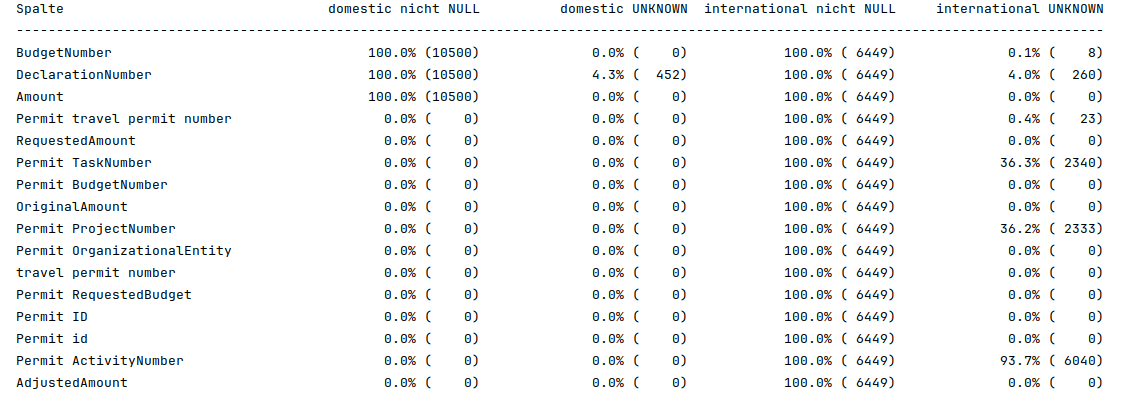
\includegraphics[width=\textwidth]{figures/python/attribute}
    \caption{}
\end{figure}
\begin{wrapfigure}{r}{0.45\textwidth}
    \centering
    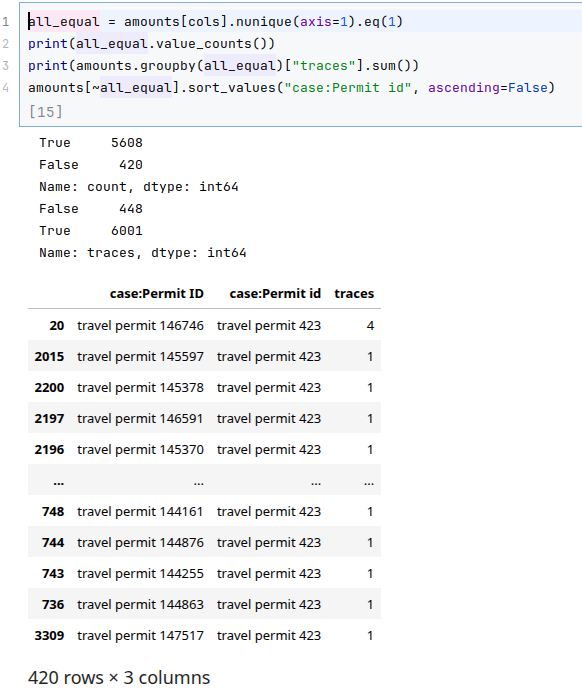
\includegraphics[width=0.45\textwidth]{figures/python/permitid}
    \caption{}
    \label{fig:permitid}
\end{wrapfigure}
Zudem gibt es in der Vielzahl der Eigenattribute von International semantische Ähnlichkeiten, die untersucht wurden.
'Permit ID' und 'Permit id' unterscheiden sich nur in der Groß-/Kleinschreibung.
Bei der Betrachtung der enthaltenen Werte, zeigt sich, dass überwiegend diese übereinstimmen, allerdings 448 Fälle existieren, in denen 'Permit id' abweichend von 'Permit ID' den Wert 'travel permit 423' enthält.
Der Wert 'travel permit 423' ist dabei nicht nur für den Fall relevant, sondern wird auch für einen Trace mit 'Permit ID' = 'travel permit 423' verwendet, wo damit eine Übereinstimmung vorliegt.
Auf eine mögliche Erklärung dieser 448/449 Fälle wird in Kapitel \todo{Kapitellink} eingegangen.
Auch die Amount-Felder 'Amount' / 'RequestedAmount' / 'AdjustedAmount' / 'OriginalAmount' wurden zusammen untersucht und zusätzlich mit 'Permit RequestedBudget' gegenübergestellt.
Es konnte festgestellt werden dass in 6448 von 6449 Fällen die ersteren 4 Felder den gleichen Wert enthalten bei 6001 verschiedenen Wertkombinationen, während zu RequestedBudget nur 24 Traces eine Gleichheit gefunden werden konnte, davon 21 Fälle mit dem Amount 0.
'case:Permit travel permit number' und 'case:travel permit number' sind in 5970 Fällen identisch und weichen in 479 Fällen voneinander ab.
'case:id' und 'case:concept:name' sind in beiden Logs je Trace immer identisch und eindeutig.
\begin{table}[htbp]
    \centering
    \caption{Attribute und Anzahl distinkter Werte je Log}
    \label{tab:attribut-maechtigkeiten}
    \footnotesize
    \setstretch{1}
    \renewcommand{\arraystretch}{1.15}
    \begin{tabularx}{\textwidth}{@{}p{2cm}XX@{}}
        \toprule
        & \textbf{Domestic (10.500 Traces)} & \textbf{International (6.449 Traces)} \\
        \midrule
        Gemeinsame Attribute
        & \texttt{id}: 56.437\par
          \texttt{org:resource}: 2\par
          \texttt{concept:name}: 17\par
          \texttt{time:timestamp}: 45.403\par
          \texttt{org:role}: 7\par
          \texttt{case:id}: 10.500\par
          \texttt{case:concept:name}: 10.500\par
          \texttt{case:BudgetNumber}: 1\par
          \texttt{case:DeclarationNumber}: 10.049\par
          \texttt{case:Amount}: 8.326
        & \texttt{id}: 69.073\par
          \texttt{org:resource}: 2\par
          \texttt{concept:name}: 34\par
          \texttt{time:timestamp}: 51.270\par
          \texttt{org:role}: 8\par
          \texttt{case:id}: 6.449\par
          \texttt{case:concept:name}: 6.449\par
          \texttt{case:BudgetNumber}: 719\par
          \texttt{case:DeclarationNumber}: 6.190\par
          \texttt{case:Amount}: 6.100 \\
        \midrule
        Log-spezifische Attribute
        & /
        & \texttt{case:Permit travel permit number}: 5.596\par
          \texttt{case:RequestedAmount}: 6.100\par
          \texttt{case:Permit TaskNumber}: 6\par
          \texttt{case:Permit BudgetNumber}: 207\par
          \texttt{case:OriginalAmount}: 6.100\par
          \texttt{case:Permit ProjectNumber}: 825\par
          \texttt{case:Permit OrganizationalEntity}: 27\par
          \texttt{case:travel permit number}: 6.033\par
          \texttt{case:Permit RequestedBudget}: 5.259\par
          \texttt{case:Permit ID}: 6.028\par
          \texttt{case:Permit id}: 5.608\par
          \texttt{case:Permit ActivityNumber}: 145\par
          \texttt{case:AdjustedAmount}: 6.101 \\
        \bottomrule
    \end{tabularx}
\end{table}

\subsection{Event-Daten}
In beiden Logs enthält ein Event die gleichen 5 Attribute: 'id', 'org:resource', 'concept:name', 'time:timestamp' und 'org:role'.
'id' und 'time:timestamp' sind Metadaten zu dem betroffenen Event.
'concept:name' beschreibt die durchgeführte Aktivität.
'org:resource' erklärt den Ursprung des Events, ob SYSTEM oder STAFF MEMBER, während 'org:role' die Rolle des Event-Akteurs wiedergibt.
Jedem möglichen Wert von 'concept:name' ist eine eindeutige Kombination aus 'org:resource' und 'org:role' zugeordnet.
\begin{figure}
    \centering
    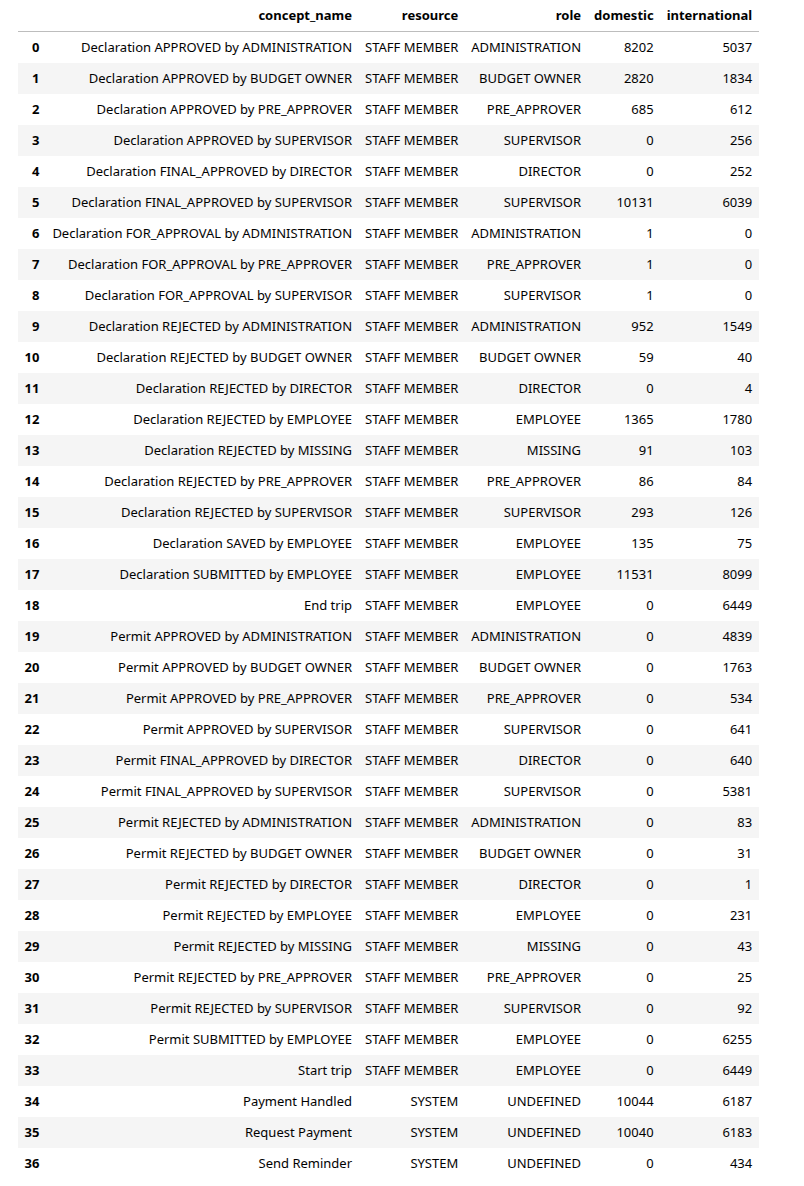
\includegraphics[width=0.7\linewidth]{figures/python/eventtypes}
    \caption{}
    \label{fig:eventtypes}
\end{figure}
Bei Domestic sind alle im Log enthaltenen Events in ihrer id eindeutig, während bei International einzelne Events (Kennung über id und time:timestamp) mehrfach vorkommen.
Dies betrifft 1480 Event-Ids mit insgesamt 4558 Nennungen.
Eine Abweichung des Timestamps oder des concept:name innerhalb der gleichen Event-Id gibt es bei allen Nennungen in dem Log nicht, weswegen von dem selben Event ausgegangen werden kann.
Mit einer Differenz von 3078 ($4558-1480$) IDs wird der Unterschied der initialen 72.151 Events (Tabelle \ref{tab:basisstatistik}) zu den 69.073 distinkten Event-Ids in \todo{\ref{tab:attribut-maechtigkeiten}} erklärt.

	\section{Prozessfluss und allgemeiner Ablauf}
\label{sec:prozessfluss}
Die beiden Event-Logs bilden je einen Genehmigungsprozess für Reisen und deren Kostenabdeckung ab, unterscheiden sich jedoch im konkreten Ablauf.
Nach Tabelle \ref{tab:basisstatistik} und \ref{fig:eventtypes} kommen 17 bzw. 34 verschiedene Ereignisse vor, wobei die Vereinigungsmenge eine Mächtigkeit von 37 beträgt.
Mit menschlicher Sicht werden schnell bestimmte Eventgruppen sichtbar, die inhaltlich zusammengehören (z.B. Trip-Events, Permit-Events), oder auch Muster in der Benennung des concept:name erkennbar.
Um dies maschinell zu untersuchen, werden die 37 Eventnamen als Text mit Python verarbeitet.
Dafür werden die Eventnamen zu Wortlisten anhand des Leerzeichens zerlegt und anschließend Cluster gebildet anhand aller verwendeten Wörter und der Menge der Übereinstimmungen zwischen zwei Namen.
25 Cluster konnten so identifiziert werden, mit Elementanzahlen von 1 bis 34.
Für die einzelnen Cluster wird ein Pattern automatisiert identifiziert, der alle Elemente des Clusters beschreibt.
Cluster mit leeren Patterns oder einem 'allMatch'-Ausdruck wurden verworfen, da sie keine inhaltliche Aussagekraft besitzen.
Mithilfe des 'Algorithmus X' von Donald Knuth \todo{Quelle} wird ein Exact-Cover-Problem der Cluster angegangen und damit Clustermengen identifiziert, bei denen jedes der 37 Events genau einmal eindeutig identifiziert und somit einem Cluster zugeordnet wird.
Es entstehen 12 übrige Filterfunktionen, um jedes Event einer eindeutigen Äquivalenzklasse zuzuordnen.
\begin{wrapfigure}{r}{0.5\textwidth}
    \centering
    \vspace{-0.7cm}
    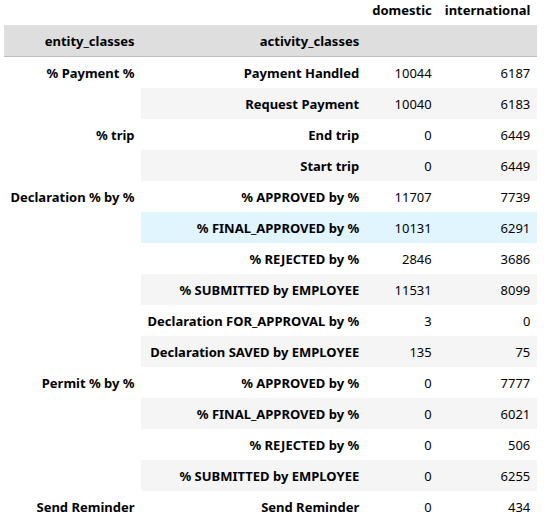
\includegraphics[width=0.5\textwidth]{figures/python/filters}
    \caption{Eventeinteilung je Log nach Filterfunktionen unter Angabe des zugehörigen Patterns}
    \label{fig:filters}
\end{wrapfigure}
Die inhaltliche Bedeutung dieser Relationen wird mit Domänenwissen menschlich interpretiert, sodass Relationen mit Zusammenfassungen durch 'contains-By'-Pattern oder durch das Mischen von Aktivitäten und deren Kontext (z.B. 'Start' und 'Permit' in der gleichen Filterfunktion) entfernt werden, da sie Bedeutungsbereiche vermischen.
Übrig bleiben 2 Filterfunktionen, die Eventnamen inhaltlich einteilen und die Interpretierung von Prozessen unterstützen:
\begin{itemize}
    \item Filterfunktion 'entity\_classes': [DECLARATION, PERMIT, PAYMENT, TRIP, REMINDER SEND]
    \item Filterfunktion 'activity\_classes': [REJECTED, APPROVED, FINAL\_APPROVED, FOR\_APPROVAL, SUBMITTED, END, HANDLED, REMINDER SEND, REQUEST, SAVED, START]
\end{itemize}
% Umfang: 2-3 Seiten
% Assignment-Frage 1: Describe and visualize the general underlying process flow.
%   Reasonable level of abstraction. BPMN / Petri Nets.
% Assignment-Frage 7 (teilweise): Unterschiede International vs. Domestic.
% Quellen: Process Discovery \parencite{leemans_discovering_2013,augusto_automated_2019},
%          BPMN \parencite{dumas_fundamentals_2018}

\subsection{Domestic Declarations}
\label{sec:prozessfluss_domestic}
Bereits absehbar an Abb. \ref{fig:filters} ist, dass im Domestic-Log die Eventgruppen 'Permit', 'Trip' und 'Reminder Send' nicht vorkommen, sodass die Prozessidentifikation sich auf Declaration- und Payment-Aktivitäten konzentrieren kann.
\begin{wrapfigure}{r}{0.55\textwidth}
    \centering
    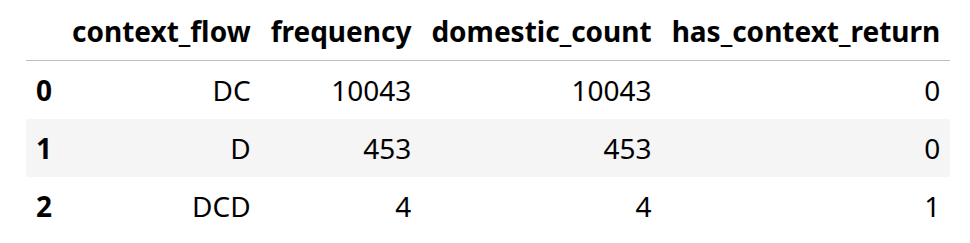
\includegraphics[width=0.55\textwidth]{figures/python/DomesticClasses}
    \caption{Entitätsklassenablauf im Domestic-Log (D=Declaration, C=Payment)}
    \label{fig:domesticclasses}
\end{wrapfigure}
Mithilfe der Filterfunktion 'entity\_classes' und Beschränkungen auf Klassenwechseln wird ersichtlich, dass die Payment-Aktivitäten im Domestic-Log immer gebündelt und nie zu Beginn stattfinden (s. Abb. \ref{fig:domesticclasses}) - in nur 4 der 10500 Fälle wird eine Declaration-Aktion noch erneut nach dem Payment durchgeführt.

% Celonis-Notizen:
%   Cases: 4618 happy path, 10500 total (43,98 %)
%   Happy-Path-TPT: 9 d
%   Algorithmischer Happy Path:
%     Declaration SUBMITTED by EMPLOYEE -> Declaration APPROVED by ADMINISTRATION
%     -> Declaration FINAL_APPROVED by SUPERVISOR -> Request Payment -> Payment Handled
%   Varianten: 100
% Abbildung: BPMN-Export aus Celonis (resources/CelonisDomesticDeclarations.bpmn
%            -> als PDF/PNG nach figures/celonis/ exportieren)

\todo{Abbildung BPMN Domestic (figures/celonis/) und Beschreibung}

\subsection{International Declarations}
\label{sec:prozessfluss_international}

% Celonis-Notizen:
%   Cases: 1369 happy path, 6449 total (21,23 %)
%   Happy-Path-TPT: 66 d
%   Algorithmischer Happy Path:
%     Permit SUBMITTED by EMPLOYEE -> Permit APPROVED by ADMINISTRATION
%     -> Permit FINAL_APPROVED by SUPERVISOR -> Start trip -> End trip
%     -> Declaration SUBMITTED by EMPLOYEE -> Declaration APPROVED by ADMINISTRATION
%     -> Declaration FINAL_APPROVED by SUPERVISOR -> Request Payment -> Payment Handled
%   Varianten: 756
% Abbildung: BPMN-Export aus Celonis (resources/CelonisInternationalDeclarations.bpmn)

\todo{Abbildung BPMN International (figures/celonis/) und Beschreibung}

\subsection{Abstraktionsniveau und Vergleich}
\label{sec:prozessfluss_vergleich}

% - Abstraktion begründen: Varianten-Abdeckung (Top-n-Varianten = x % der Cases),
%   Frequenzfilter im Process Explorer.
% - International = Domestic-Kern + vorgelagerte Permit-Phase + Trip-Events.
% - Optional: Inductive-Miner-Modell aus PM4Py (Jesco, figures/python/) gegenüberstellen.

\todo{Vergleich Domestic vs. International; ggf. PM4Py-Modell von Jesco}

	\section{Performance- und Konformitätsanalyse}
\label{sec:performance}

Aufbauend auf dem in \autoref{sec:prozessfluss} rekonstruierten Prozessfluss untersucht dieses Kapitel die Prozessleistung und -konformität:
Wie lange dauern die Prozessinstanzen, wo entstehen operative Engpässe, wie häufig und warum werden Anträge abgelehnt und an welchen Stellen
weicht das beobachtete Verhalten vom erwarteten Ablauf ab. Die Untersuchung stützt sich auf die Standard-Analysen
der Celonis-Process-Analytics-Umgebung (\textit{Process Overview}, \textit{Throughput Times}, \textit{Conformance} und \textit{Process AI})
sowie auf eigens erstellte interaktive Analyse-Views (\textit{Case Explorer}, \textit{Variant Explorer} und \textit{Rejections Dashboard}),
deren Kennzahlen über die Process Query Language (PQL) aggregiert werden \parencite{vogelgesang_celonis_2022}. Zur methodischen Validierung
werden die Ergebnisse an zentralen Stellen den Python-Auswertungen mit PM4Py gegenübergestellt \parencite{berti_process_2019}. \autoref{tab:kpi_comparison}
fasst die wichtigsten Performance- und Konformitätskennzahlen beider Event-Logs zusammen.

\begin{table}[htbp]
\centering
\caption{Zentrale Performance- und Konformitätskennzahlen (Celonis)}
\label{tab:kpi_comparison}
\small
\begin{tabular*}{\textwidth}{@{\extracolsep{\fill}} l c c @{}}
\toprule
\textbf{Kennzahl} & \textbf{Domestic} & \textbf{International} \\ \midrule
Cases gesamt & 10.500 & 6.449 \\
Ø Durchlaufzeit Happy Path (Median) & 9\,d (7\,d) & 66\,d (55\,d) \\
Ø Durchlaufzeit alle Cases ohne Extreme (Median) & 9\,d (7\,d) & 75\,d (66\,d) \\
Ø Durchlaufzeit alle Cases inkl.\ Extreme & 11,5\,d (bis 469\,d) & 86\,d (bis 743\,d) \\
Ø Dauer Deklarationsteil (\texttt{SUBMITTED} $\rightarrow$ \texttt{Payment}) & 11,6\,d (Median: 7,4\,d) & 14,6\,d (Median: 10,2\,d) \\
Konforme Cases: Striktes Modell (nur Variante 1) & 43,98\,\% (4.618) & 21,23\,\% (1.369) \\
Konforme Cases: Erweitertes Modell (Top-3-Varianten) & 81,00\,\% (8.470) & 38,30\,\% (2.470) \\
Verletzungstypen (im erweiterten Modell) & 19 & 56 \\
Ø Durchlaufzeit konform vs.\ verletzend (erw.\ Modell) & 10,4 vs.\ 16,3\,d (+5,9\,d) & 69,3 vs.\ 97,1\,d (+27,8\,d) \\
Schritte pro Case konform vs.\ verletzend (erw.\ Modell) & 5,1 vs.\ 6,4 & 10,2 vs.\ 11,8 \\
Cases mit mindestens einer Ablehnung (Gesamtquote) & 1.301 (12\,\%) & 1.755 (27\,\%) \\
\quad davon \texttt{Declaration REJECTED by EMPLOYEE} & 1.212 (12\,\%), +9\,d & 1.483 (23\,\%), +18\,d \\
\quad davon \texttt{Declaration REJECTED by ADMINISTRATION} & 846 (8\,\%), +11\,d & 1.287 (20\,\%), +15\,d \\
\quad davon \texttt{Declaration REJECTED by SUPERVISOR} & 281 (3\,\%), +9\,d & 211 (3\,\%), +12\,d \\
Wiederholte Einreichung (\texttt{SUBMITTED} $\rightarrow$ \texttt{SUBMITTED}) & 776 (7\,\%), +12\,d & 1.225 (19\,\%), +20\,d \\ \bottomrule
\end{tabular*}
\end{table}

% ==================================================================
\subsection{Durchlaufzeiten und Extremwertanalyse}
\label{sec:durchlaufzeiten}

\paragraph{International.} Die arithmetische Gesamtdurchlaufzeit vom ersten bis zum letzten Event eines internationalen Abrechnungsfalls beträgt 86 Kalendertage.
Wie das Histogramm in \autoref{fig:tpt_verteilung} zeigt, ist die Verteilung stark rechtsschief: Während sich die Mehrheit der Fälle (rund 4.200 Cases) in den
ersten drei Intervallen zwischen 7 und 86 Tagen konzentriert, fällt die Häufigkeit danach kontinuierlich ab, mündet jedoch am rechten Rand in einer Sammelklasse
extremer Ausreißer von 224 bis zu 743 Tagen (rund 360 Cases). Dieser ausgeprägte \textit{Long Tail} zieht das arithmetische Mittel signifikant nach oben.
In den Standard-Dashboards von Celonis werden daher drei unterschiedlich aggregierte Durchschnittswerte ausgewiesen, die analytisch strikt zu trennen sind:

\begin{itemize}[noitemsep]
	\item \textbf{86 Tage:} ungefiltertes arithmetisches Mittel \emph{aller} 6.449 Cases inklusive sämtlicher Ausreißer (Tab \textit{Throughput Times} in Process Overview),
	\item \textbf{75 Tage:} getrimmtes Mittel aller Cases \emph{ohne Extremwerte} (View \textit{Process Overview}),
	\item \textbf{66 Tage:} arithmetisches Mittel ausschließlich der 1.369 Happy-Path-Cases (Variante 1).
\end{itemize}

Für eine gegenüber Ausreißern robuste Bewertung ist der Median heranzuziehen:
Dieser liegt über alle internationalen Fälle hinweg bei 66 Tagen und reduziert sich für die Fälle auf dem Happy Path auf 55 Tage.

\paragraph{Domestic und 0-ms-Anomalie.} Inländische Deklarationen werden um ein Vielfaches schneller abgewickelt. Sowohl auf dem Happy Path als
auch im getrimmten Gesamtdurchschnitt beträgt die mittlere Durchlaufzeit 9 Kalendertage, sodass der Großteil der Erstattungen innerhalb von knapp
zwei Wochen abgeschlossen ist.

Eine gezielte Untersuchung der Varianten-Tabelle im selbsterstellten Celonis-View (\autoref{fig:view_variants} im Anhang) deckt jedoch zwei extreme
Auffälligkeiten an den Rändern der Verteilung auf:
\begin{enumerate}[noitemsep]
	\item \textbf{Fälle mit 0\,ms Durchlaufzeit (Variante 8):} Exakt 134 Domestic-Cases (1\,\%) weisen eine gemessene Durchlaufzeit von 0 Millisekunden auf. Eine Einzelfallprüfung im \textit{Case Explorer} zeigt, dass diese Traces aus lediglich einem einzigen Event (\texttt{Declaration SAVED by EMPLOYEE}) bestehen. Fachlich handelt es sich um Entwürfe, die von Mitarbeitenden im System zwischengespeichert, aber nie formal eingereicht wurden. Verbleiben diese unvollständigen Instanzen ungefiltert im Log, verzerren sie sowohl die durchschnittliche Durchlaufzeit als auch die Schrittanzahl künstlich nach unten.
	\item \textbf{Extreme Langläufer durch Liegezeiten (bis 283 Tage):} Am oberen Ende finden sich auch im Domestic-Log gravierende Ausreißer. Eine im \textit{Case Explorer} durchgeführte Einzelfallanalyse des Extremfalls \texttt{f954cbea-975d-4cf4-a1f6-a400d81f0d9f} (Durchlaufzeit: 283 Tage, 9 Aktivitäten; siehe \autoref{fig:case_f954} im Anhang) verdeutlicht die Ursache: Nachdem die Erklärung am 04.12.2017 eingereicht wurde, verblieb sie fast neun Monate ohne jegliche Systemaktivität, ehe sie am 27.08.2018 von der Administration abgelehnt wurde. Nach der erneuten Einreichung am 10.09.2018 wurde der gesamte restliche Freigabe- und Auszahlungsprozess (inklusive Budget Owner und Supervisor) innerhalb von nur drei Tagen bis zum 13.09.2018 abgeschlossen. Die extremen Durchlaufzeiten resultieren folglich nicht aus komplexen Bearbeitungen, sondern aus monatelang verwaisten Anträgen, die zudem jahresübergreifende Events erzeugen.
\end{enumerate}

\paragraph{Vergleichbarkeit der beiden Logs.}
Die Gesamtdurchlaufzeiten von rund 9 Tagen (Domestic) und 66 bzw.\ 86 Tagen (International) lassen sich nicht direkt miteinander vergleichen, da beide Logs unterschiedliche Prozessgrenzen abbilden: Während ein Domestic-Case erst mit \texttt{Declaration SUBMITTED by EMPLOYEE} startet, umfasst ein International-Case zusätzlich die gesamte Permit- und Reisephase. Um einen methodisch fairen Vergleich herzustellen, wurde im eigens erstellten Analyse-Tab \textit{TPT Analysis} exakt derselbe Prozessabschnitt vom ersten Einreichen der Erklärung (\texttt{Declaration SUBMITTED by EMPLOYEE}, \textit{First}) bis zum Zahlungsabschluss (\texttt{Payment Handled}, \textit{Last}) für beide Logs isoliert ausgewertet (\autoref{fig:view_compare_dec}).

Das Ergebnis relativiert den scheinbar massiven Geschwindigkeitsunterschied erheblich: Im Domestic-Log benötigt dieser Abschnitt über alle ausgezahlten Fälle hinweg im ungetrimmten Mittel 11,6 Tage bei einem Median von 7,41 Tagen (Minimum: 1,06 Tage, Maximum: 368 Tage). Im International-Log liegt das arithmetische Mittel für denselben Abschnitt bei 14,6 Tagen und der Median bei 10,2 Tagen (Minimum: 1,09 Tage, Maximum: 429 Tage). Die eigentliche Prüfung, Freigabe und Auszahlung einer Auslandsabrechnung dauert im Schnitt folglich nur rund 3,0 Tage (im Median 2,8 Tage) länger als bei einer Inlandsreise – ein moderater Aufschlag, der sich durch die höhere Komplexität ausländischer Belege und die höhere Korrekturquote erklärt. Die übrigen mehr als 70 Tage Differenz in der Gesamtdurchlaufzeit entfallen vollständig auf die vorgelagerte Permit-Genehmigung, die Buchungsvorlaufzeit, die Reisedauer sowie das verzögerte Einreichen nach Rückkehr.

\begin{figure}[htbp]
	\centering
	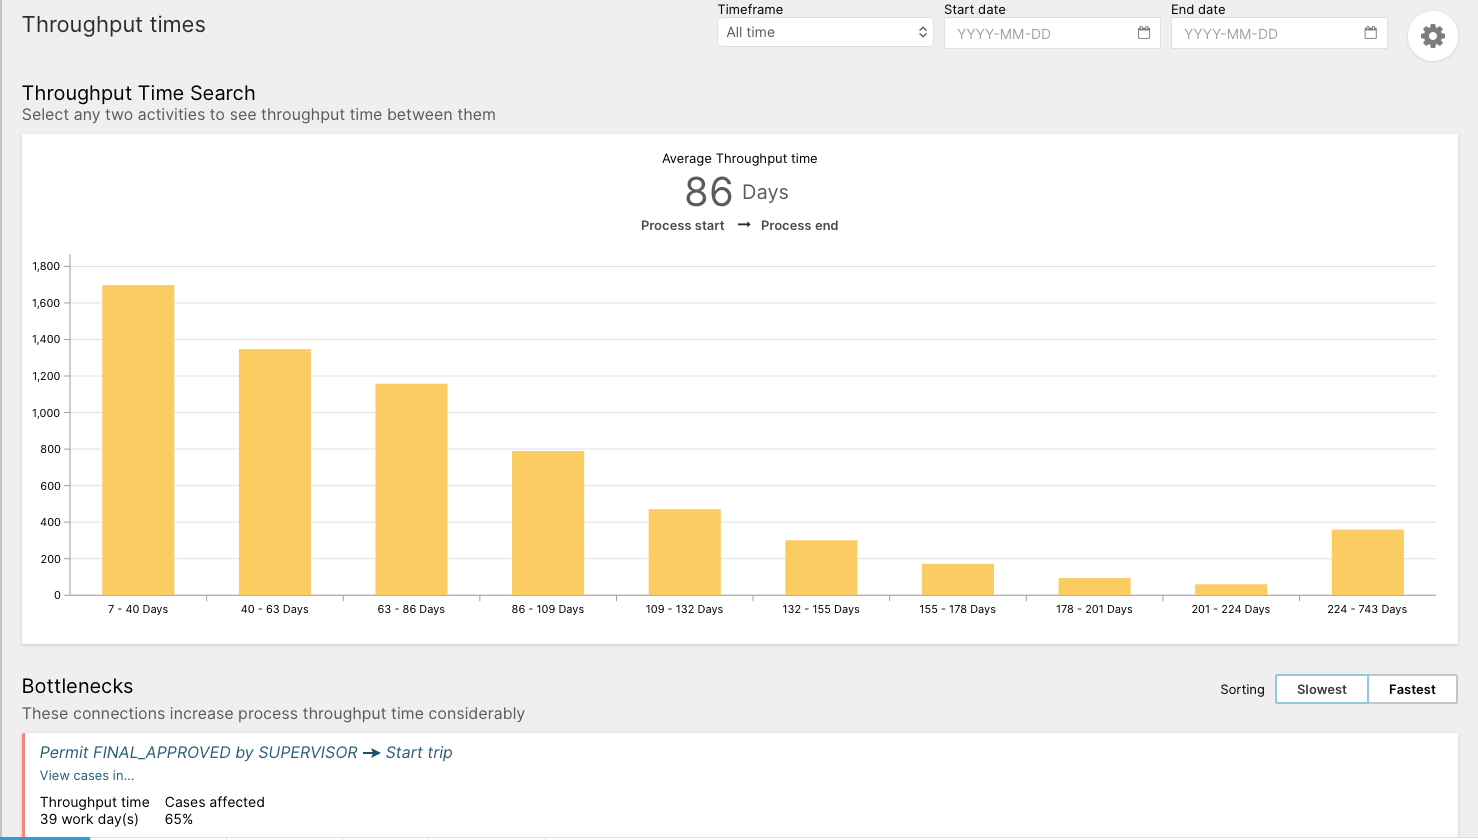
\includegraphics[width=0.85\textwidth]{figures/celonis/int_throughput.png}
	\caption{Rechtsschiefe Verteilung der Durchlaufzeiten mit Long Tail bis 743 Tage (International, Celonis \textit{Throughput Times})}
	\label{fig:tpt_verteilung}
\end{figure}

\paragraph{Zeitliche Muster.} Die Anzahl neu gestarteter Fälle pro Monat unterliegt im Beobachtungszeitraum einem markanten Strukturbruch. Im International-Log starten im Jahr 2017 durchschnittlich rund 10 Cases pro Tag; ab Januar 2018 vervielfacht sich dieser Wert sprunghaft auf bis zu 55 Starts pro Tag im April 2018. Dasselbe Muster zeigt sich im Domestic-Log mit 2.240 Case-Starts im Jahr 2017 gegenüber 8.345 im Jahr 2018 (\autoref{tab:basisstatistik}). Wie in \autoref{sec:einleitung} erläutert, ist dieser Anstieg kein Ausdruck einer veränderten Reisetätigkeit, sondern das direkte Resultat des universitätsweiten System-Rollouts Anfang 2018 \parencite{van_dongen_bpi_2020}. Ab Anfang 2019 (301 Domestic- bzw.\ 176 International-Starts) läuft die Erfassung neuer Fälle aus, während einzelne Bearbeitungs-Events bis 2020 nachlaufen. Methodisch führt dies an den Rändern des Beobachtungsfensters zu einer statistischen Verzerrung: Fälle aus 2017 hatten bis zum Datenexport über zwei Jahre Zeit, um selbst extremste Liegezeiten (wie im obigen 283-Tage-Fall) vollständig im Log abzubilden, wohingegen spät im Jahr 2018 gestartete Fälle bei einer kurzen Abwicklung bevorzugt im Log abgeschlossen sind (Rechtszensierung langer Fälle).

% ==================================================================
\subsection{Bottlenecks}
\label{sec:bottlenecks}

Die Bottleneck-Analyse in Celonis identifiziert diejenigen direkten Aktivitätsübergänge, welche die Gesamtdurchlaufzeit am stärksten verzögern (\autoref{fig:bottlenecks}).

\paragraph{Domestic.} Innerhalb des Genehmigungsworkflows sind die Liegezeiten mit ein bis zwei Arbeitstagen ausgesprochen kurz. Die beiden gravierendsten Engpässe treten erst nach Abschluss sämtlicher inhaltlicher Prüfungen in der finalen Zahlungsabwicklung auf: Der Übergang \texttt{FINAL\_APPROVED by SUPERVISOR \textrightarrow\ Request Payment} beansprucht im Mittel 3 Arbeitstage (96\,\% der Cases), gefolgt von \texttt{Request Payment \textrightarrow\ Payment Handled} mit weiteren 4 Arbeitstagen (95\,\% der Cases). Damit entfallen rund sieben Arbeitstage – und somit der überwiegende Teil der neuntägigen Happy-Path-Durchlaufzeit – auf die rein technische Auszahlungsphase. Da diese Aktivitäten vom Akteur \texttt{SYSTEM} ausgeführt werden, deutet dieses Muster stark darauf hin, dass Zahlungsanweisungen und Überweisungsläufe im Finanzsystem der Universität nicht in Echtzeit, sondern gebündelt in wöchentlichen oder halbwöchentlichen Batch-Läufen prozessiert werden. Als drittgrößter Verzögerungsfaktor erweist sich der Übergang \texttt{APPROVED by BUDGET OWNER \textrightarrow\ FINAL\_APPROVED by SUPERVISOR} (3\,AT in 26\,\% der Cases), was bestätigt, dass die zusätzliche Hierarchiestufe des Budgetverantwortlichen die Prozessdauer spürbar erhöht.

\paragraph{International.} Im Auslandsprozess weist Celonis rechnerisch den Übergang \texttt{Permit FINAL\_APPROVED by SUPERVISOR \textrightarrow\ Start trip} mit 39 Arbeitstagen (65\,\% der Cases) als langsamsten Prozessschritt aus. Fachlich stellt diese Zeitspanne jedoch keinen operativen Prozessengpass dar, sondern spiegelt die notwendige und erwünschte Vorlaufzeit zwischen der Genehmigung einer Auslandsdienstreise und dem tatsächlichen Reiseantritt wider. Analog bildet der Übergang \texttt{Start trip \textrightarrow\ End trip} (5\,AT, 90\,\%) schlicht die physische Dauer der Dienstreise ab. Dies unterstreicht, dass algorithmisch identifizierte Liegezeiten im Process Mining stets im fachlichen Domänenkontext interpretiert werden müssen.

Der tatsächliche operative Flaschenhals im International-Log liegt im Übergang \texttt{End trip \textrightarrow\ Declaration SUBMITTED by EMPLOYEE}, der bei 71\,\% der Fälle im Mittel 13 Arbeitstage (rund drei Kalenderwochen) beansprucht. Diese Verzögerung entsteht vollständig aufseiten der reisenden Mitarbeitenden, die ihre Belege nach Rückkehr erst mit erheblichem Verzug einreichen. Die nachgelagerte Zahlungsphase (\texttt{Request Payment \textrightarrow\ Payment Handled}, 3\,AT, 95\,\%) verhält sich hingegen konsistent zum Inlandsprozess. Auffällig ist zudem der zweitlangsamste Übergang \texttt{Permit FINAL\_APPROVED by SUPERVISOR \textrightarrow\ Declaration SUBMITTED by EMPLOYEE} (17\,AT, 12\,\% der Cases), bei dem die Reise-Events zwischen Permit-Freigabe und Kostenerklärung komplett fehlen; diese Konformitätsanomalie wird in \autoref{sec:unerwartet} aufgelöst.

\begin{figure}[htbp]
	\centering
	\begin{subfigure}[t]{0.49\textwidth}
		\centering
		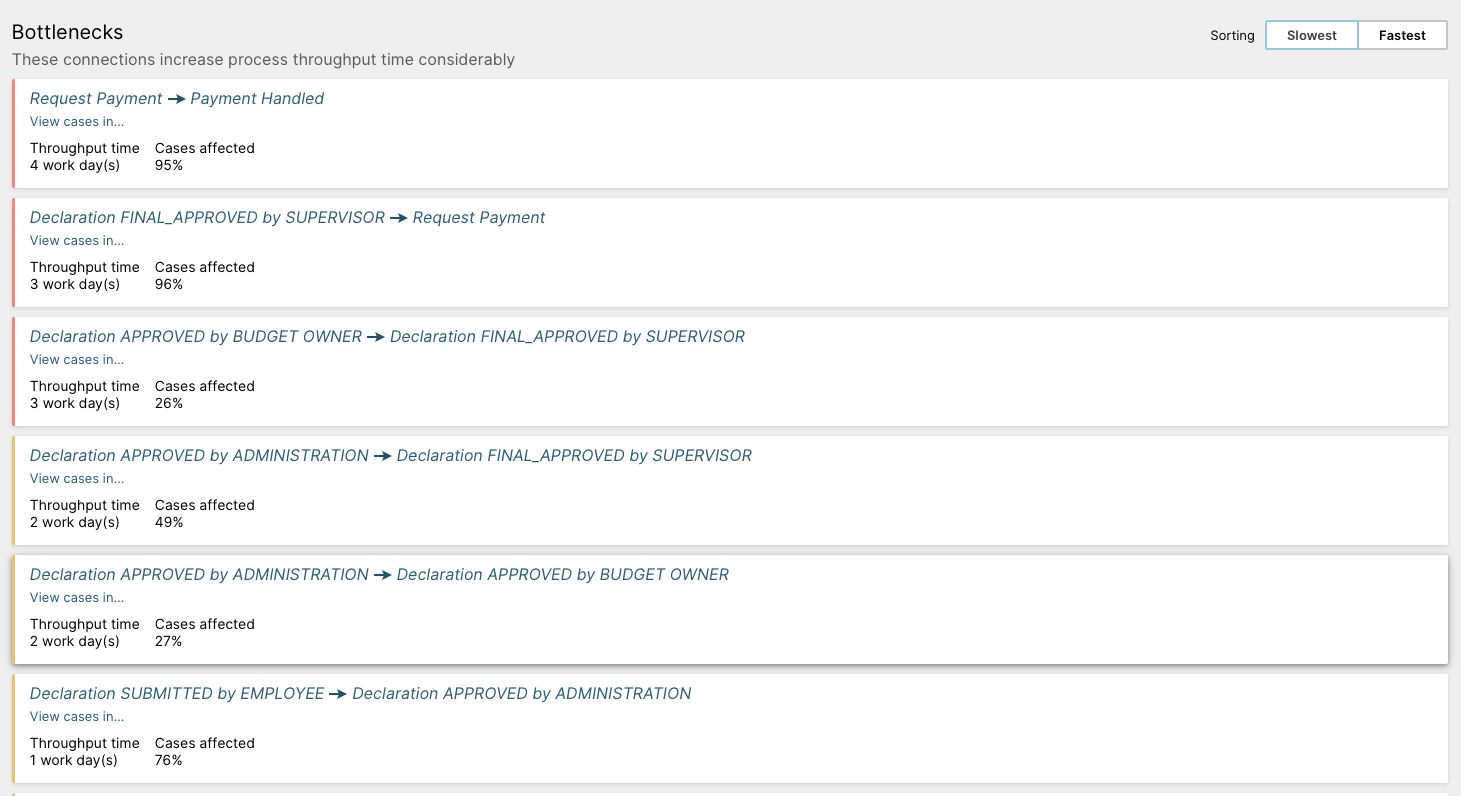
\includegraphics[width=\textwidth]{figures/celonis/dom_bottlenecks.png}
		\caption{Domestic}
	\end{subfigure}
	\hfill
	\begin{subfigure}[t]{0.49\textwidth}
		\centering
		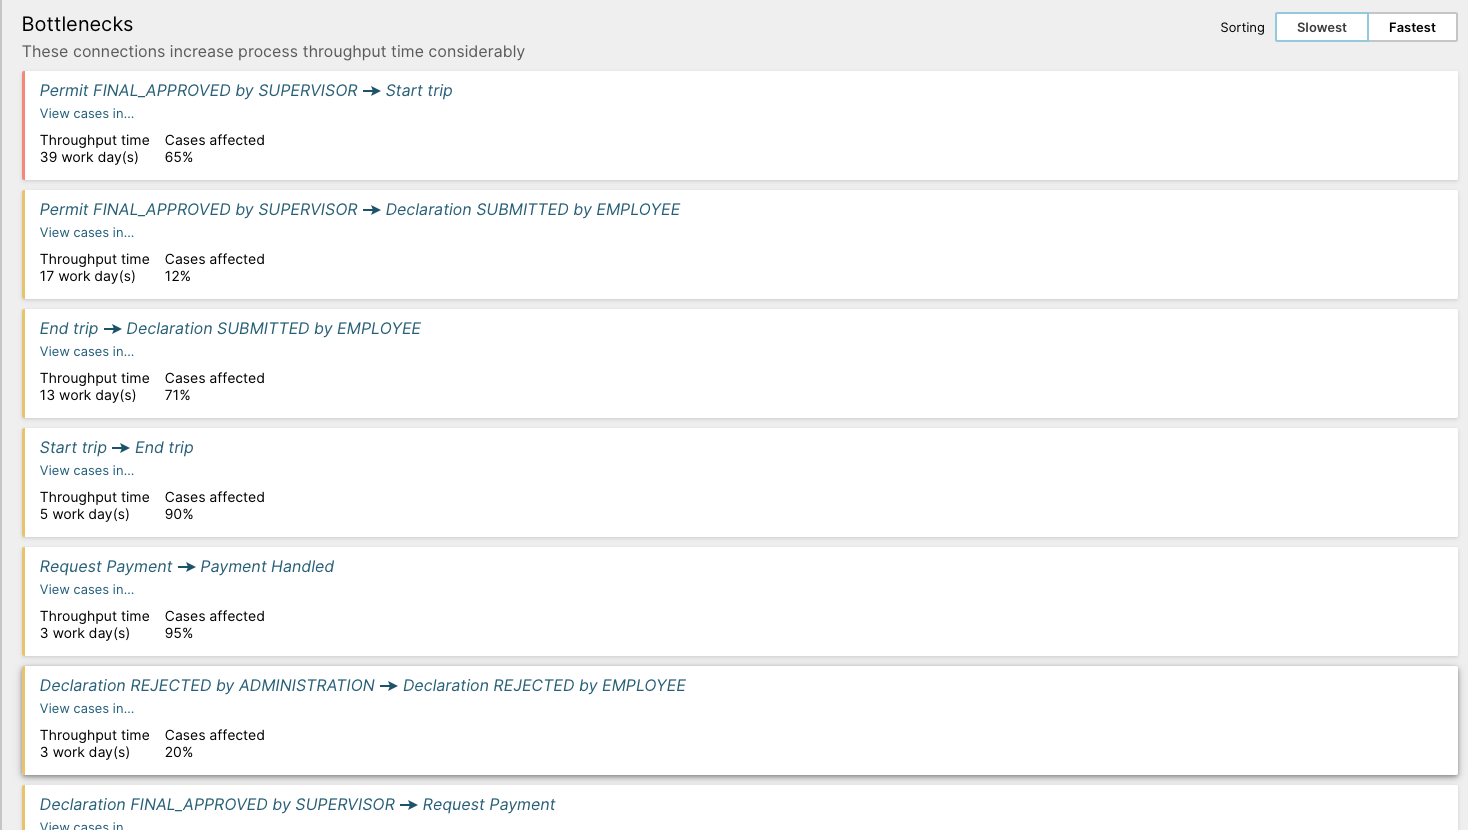
\includegraphics[width=\textwidth]{figures/celonis/int_bottlenecks.png}
		\caption{International}
	\end{subfigure}
	\caption{Langsamste Aktivitätsübergänge laut Celonis-Bottleneck-Analyse (in Arbeitstagen)}
	\label{fig:bottlenecks}
\end{figure}

% ==================================================================
\subsection{Ablehnungen und Rework-Schleifen}
\label{sec:rejections}

Die Auswertung im eigens konzipierten \textit{Rejections Dashboard} (siehe \autoref{fig:view_rejections} im Anhang) zeigt, dass Ablehnungen ein massives Effizienzproblem darstellen: Im Domestic-Log sind insgesamt 1.301 von 10.500 Fällen (12\,\%) von mindestens einer Ablehnung betroffen; im komplexeren International-Log steigt diese Quote um mehr als das Doppelte auf 1.755 von 6.449 Fällen (27\,\%), wobei dort sowohl die vorgelagerten Permits als auch die nachgelagerten Declarations abgelehnt werden können.

Auf Ebene der prüfenden Instanzen dominiert die Verwaltung (\texttt{ADMINISTRATION}), die in 846 Domestic-Cases (8\,\%) und 1.287 International-Cases (20\,\%) eine Ablehnung ausspricht, gefolgt vom \texttt{SUPERVISOR} (281 Domestic-Cases, 3\,\%) sowie selteneren Zurückweisungen durch \texttt{PRE\_APPROVER} (81 Cases), \texttt{BUDGET OWNER} (58 Cases), \texttt{DIRECTOR} und eine nicht näher spezifizierte Rolle \texttt{MISSING} (87 Domestic-Cases). Da die Gesamtzahl der protokollierten Ablehnungs-Events die Anzahl der betroffenen Cases deutlich übersteigt (z.\,B.\ 952 Admin-Ablehnungs-Events verteilt auf 846 Cases bei Domestic bzw.\ 1.549 Events auf 1.287 Cases bei International), durchlaufen zahlreiche Anträge mehrfache Zurückweisungsschleifen.

\paragraph{Aufklärung der Aktivität \enquote{Rejected by EMPLOYEE}.}
Quantitativ tritt in beiden Logs die Aktivität \texttt{Declaration REJECTED by EMPLOYEE} mit 1.212 Fällen (12\,\%, Domestic) bzw.\ 1.483 Fällen (23\,\%, International) am häufigsten auf. Durch eine gezielte Filterung auf die 1.301 abgelehnten Domestic-Cases im selbsterstellten Celonis-View (\autoref{fig:view_rejections} im Anhang) lässt sich die tatsächliche Prozesssemantik dieser zunächst widersprüchlich klingenden Aktivität eindeutig klären: Sie tritt im Prozessgraphen nahezu ausnahmslos als unmittelbarer Folgeschritt nach einer Ablehnung durch die Administration, den Supervisor oder den Budget Owner auf (im International-Log im Mittel nach 3 Arbeitstagen, vgl.\ \autoref{fig:bottlenecks}). Eine Überprüfung konkreter Einzelfälle im \textit{Case Explorer} – etwa Case \texttt{ff999942-a443-4452-9b09-3c5e60ee3a8f}, bei dem exakt sieben Stunden nach \texttt{Declaration REJECTED by SUPERVISOR} das Event \texttt{Declaration REJECTED by EMPLOYEE} folgt – belegt, dass Mitarbeitende hier nicht ihren eigenen Antrag prüfen, sondern dass das Workflow-System einen vom Prüfer abgelehnten Antrag formal mit dem Status \texttt{REJECTED by EMPLOYEE} an den Einreicher zurückspielt (bzw.\ dieser die Kenntnisnahme/Stornierung bestätigt). Von diesem Knotenpunkt aus teilt sich der Prozessfluss im Dashboard in zwei Pfade: Entweder reicht der Mitarbeitende den korrigierten Antrag erneut ein (Rückwärtsschleife zu \texttt{Declaration SUBMITTED by EMPLOYEE}), oder der Prozess bricht an dieser Stelle endgültig ab.

\paragraph{Rework-Effekt und Prozessabbruch.}
Wird nach einer Ablehnung eine Korrekturschleife durchlaufen, führt dies zu erheblichem Mehraufwand (\textit{Rework}). In 776 Domestic-Cases (7\,\%) und 1.225 International-Cases (19\,\%) wird eine Deklaration mehrfach eingereicht, was die Durchlaufzeit im Mittel um 12 bzw.\ 20 Tage verlängert und 3,6 bzw.\ 4,6 zusätzliche Prozessschritte verursacht (\autoref{fig:violations}). Im Einzelfall zeigt sich in den Zeitstempeln, dass reine Formalkorrekturen nach der Wiedereinreichung oft in wenigen Sekunden von der Administration durchgewunken werden (im untersuchten Case \texttt{f954cbea...} dauerte die Freigabe nach der Zweiteinreichung exakt 6 Sekunden), die vorangegangene Schleife jedoch Wochen an Liegezeit gekostet hat.

Gleichzeitig zeigt die Filterung auf die 1.301 abgelehnten Domestic-Cases im Prozessgraphen (\autoref{fig:view_rejections} im Anhang), dass 979 dieser Fälle (75\,\% der abgelehnten Fälle) nach erfolgreicher Korrektur dennoch den Endknoten \texttt{Payment Handled} erreichen. Die verbleibenden 322 abgelehnten Fälle enden hingegen ohne Auszahlung. Zusammen mit den 134 nie eingereichten Entwürfen (\texttt{SAVED by EMPLOYEE}) erklärt dies exakt die insgesamt 456 Domestic-Cases (4,3\,\%), in denen kein \texttt{Payment Handled} stattfindet (10.044 bezahlte von 10.500 Fällen). Im International-Log bleiben analog 190 Cases ohne Auszahlung (6.259 bezahlte von 6.449 Fällen).

\paragraph{Analyse potenzieller Ablehnungsgründe.}
Inhaltliche Ablehnungsgründe (wie bspw.\ fehlende Originalbelege, falsch berechnete Tagessätze oder unzulässige Ausgabenkategorien) werden im Event-Log nicht als explizites Textattribut erfasst.
Der direkte XES-Upload in Celonis übernimmt standardmäßig lediglich die Event-Ebene (\texttt{id}, \texttt{org:resource}, \texttt{concept:name}, \texttt{time:timestamp}, \texttt{org:role}) in die zentrale Aktivitätstabelle (vgl.\ Abbildung~\ref{fig:anhang-datenmodell}).
Die auf Case-Ebene liegenden Metadaten, etwa die Betragsfelder \texttt{Amount}, \texttt{RequestedAmount}, \texttt{AdjustedAmount} oder \texttt{OriginalAmount}, stehen im Standard-Import nicht als Case-Attribute für PQL-Abfragen zur Verfügung.
Dieses Verhalten deckt sich mit einem dokumentierten Feature-Request in der Celonis Community, wonach Trace-Attribute beim XES-Import auf Event-Ebene abgeflacht werden und keine separate Case-Tabelle entsteht \parencite{buijs2019celonis}.
Diese technische Restriktion schränkt die automatisierte Ursachenanalyse in Celonis ein.
Zwar ließe sich die Einschränkung durch eine vorgelagerte Konvertierung der Ereignisprotokolle in das CSV-Format und einen strukturierten Relational-Datenimport umgehen, bei dem sämtliche Fallattribute in das Datenmodell integriert würden; diese Erkenntnis wurde im Verlauf des Analyseprozesses jedoch erst gewonnen, als die Dashboards und Kennzahlen bereits auf Basis des nativen XES-Imports etabliert waren.
Die strukturierte Untersuchung von Ablehnungsursachen musste daher auf die in Celonis nativ verfügbaren Ablaufstrukturen, Rollen und Schleifenmuster beschränkt bleiben.

% ==================================================================
\subsection{Unerwartetes Verhalten}
\label{sec:unerwartet}

\paragraph{Fehlende Reiseanträge (Missing Permits).}
Obwohl für Auslandsreisen zwingend eine Vorabgenehmigung vorgeschrieben ist, starten 748 International-Cases (12\,\%) unmittelbar mit der Aktivität \texttt{Start trip}. Diese Regelverletzung verlängert die Gesamtdurchlaufzeit im Schnitt um 29 Tage (\autoref{fig:violations}). Ein Abgleich mit den Gesamtfallzahlen präzisiert das Bild: Da überhaupt nur 6.001 der 6.449 Fälle das Event \texttt{Permit SUBMITTED by EMPLOYEE} aufweisen, existieren genau 448 Auslandsreisen (7\,\%), die den gesamten Abrechnungsprozess ohne jemals eingereichten Reiseantrag durchlaufen – exakt jene 448 Fälle, die bereits in der Attributanalyse (\autoref{sec:datensatzuebersicht}) durch den Dummy-Eintrag \enquote{\texttt{travel permit 423}} im Feld \texttt{Permit id} aufgefallen waren. In den übrigen rund 300 der 748 Fälle wird das Permit erst nach Reiseantritt eingereicht.

\paragraph{Nachträglich genehmigte Reisen.}
Selbst wenn ein Permit gestellt wird, erfolgt die Genehmigung häufig zu spät. Wie in der Bottleneck-Analyse (\autoref{sec:bottlenecks}) beobachtet, folgt in 776 International-Cases (12\,\%) auf \texttt{Permit FINAL\_APPROVED by SUPERVISOR} direkt die Einreichung der Abrechnung (\texttt{Declaration SUBMITTED by EMPLOYEE}, 17\,AT), ohne dass dazwischen Reise-Events liegen. Eine Detailprüfung der Zeitstempel dieser 776 Fälle belegt eine massive Umgehung des Kontrollprinzips:
\begin{itemize}[noitemsep]
	\item In 582 Fällen (75\,\%) war die Dienstreise (\texttt{Start trip} bis \texttt{End trip}) bereits \emph{vollständig beendet}, bevor die finale Permit-Genehmigung erteilt wurde (488 davon begannen direkt mit \texttt{Start trip}).
	\item In 53 Fällen (7\,\%) fiel die Genehmigung in den laufenden Reisezeitraum.
	\item Lediglich in 141 Fällen (18\,\%) wurde die Kostenerklärung regulär vor Reisebeginn eingereicht (etwa zur Voraberstattung gebuchter Flüge oder Konferenzgebühren).
\end{itemize}
Die Reisegenehmigung verkommt in über vier Fünfteln dieser Fälle von einer präventiven Budgetkontrolle zu einer rein bürokratischen Nachgenehmigung, die nur noch durchlaufen wird, um die Auszahlung im System freizuschalten.

\paragraph{Zusätzliche Eskalationsstufen.}
In exakt 637 International-Cases (10\,\%) treten die Aktivitäten \texttt{Permit APPROVED by SUPERVISOR} und \texttt{Permit FINAL\_APPROVED by DIRECTOR} auf. Die identische Fallzahl belegt, dass der Supervisor hier nur eine Vorprüfung vornimmt und die Endfreigabe an die Direktoratsebene eskaliert wird. Mit einer mittleren Verzögerung von +52 Tagen stellt diese Eskalationsstufe den größten einzelnen Zeittreiber im gesamten Datensatz dar (\autoref{fig:violations}).

\paragraph{Unprotokollierte Neueinreichungen.}
Im Domestic-Log folgt in 193 Fällen (2\,\%) auf eine bereits erfolgte Verwaltungsfreigabe (\texttt{Declaration APPROVED by ADMINISTRATION}) unmittelbar ein erneutes \texttt{Declaration SUBMITTED by EMPLOYEE} (+12\,d, +4,9 Schritte), ohne dass dazwischen ein Ablehnungs-Event protokolliert ist. Dies deutet darauf hin, dass Mitarbeitende bereits geprüfte Anträge aktiv zurückziehen oder nachträglich Belege nachreichen können, was den Prüfprozess von vorn anstößt.

\begin{figure}[htbp]
	\centering
	\begin{subfigure}[t]{0.49\textwidth}
		\centering
		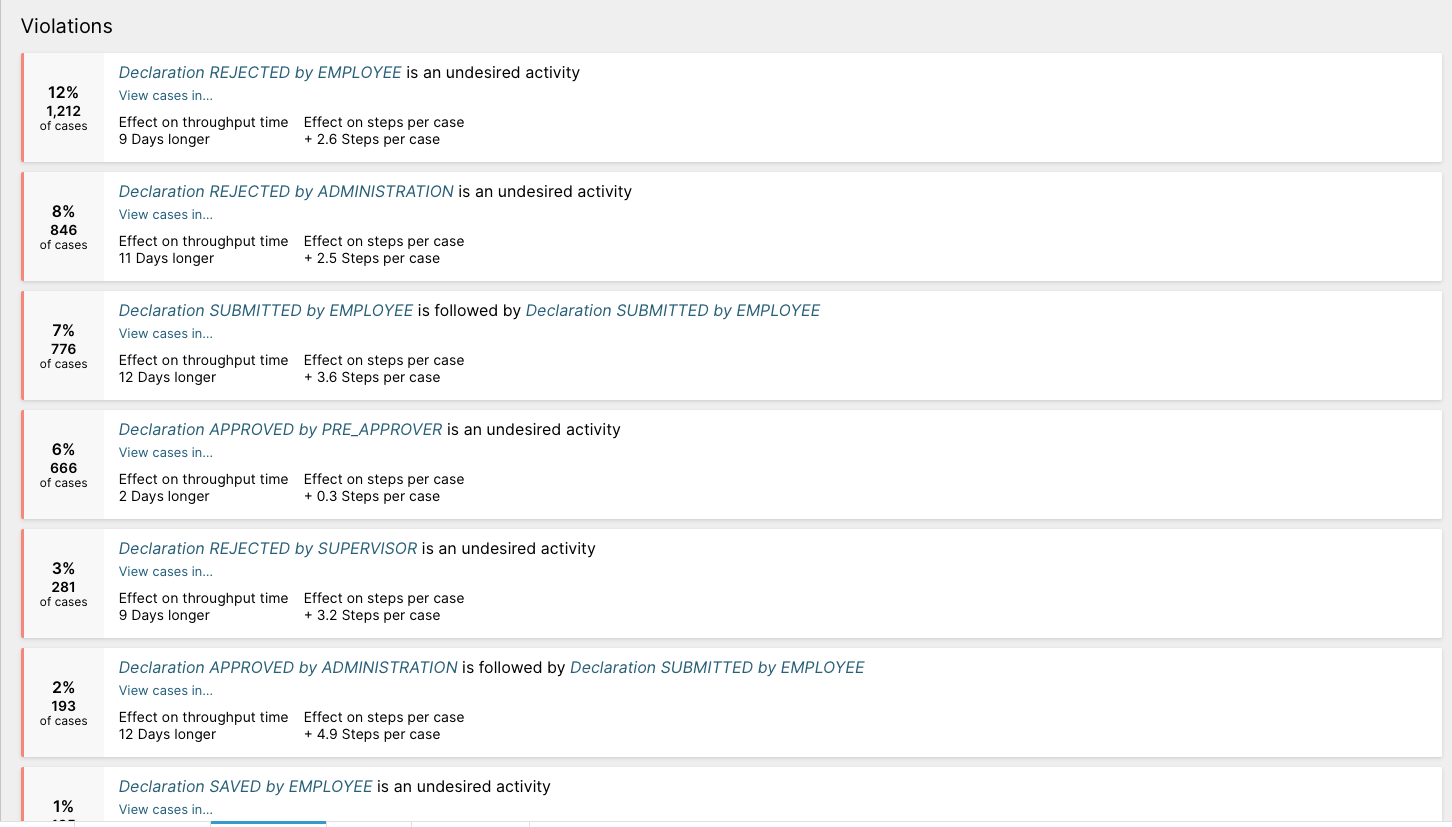
\includegraphics[width=\textwidth]{figures/celonis/dom_violations.png}
		\caption{Domestic}
	\end{subfigure}
	\hfill
	\begin{subfigure}[t]{0.49\textwidth}
		\centering
		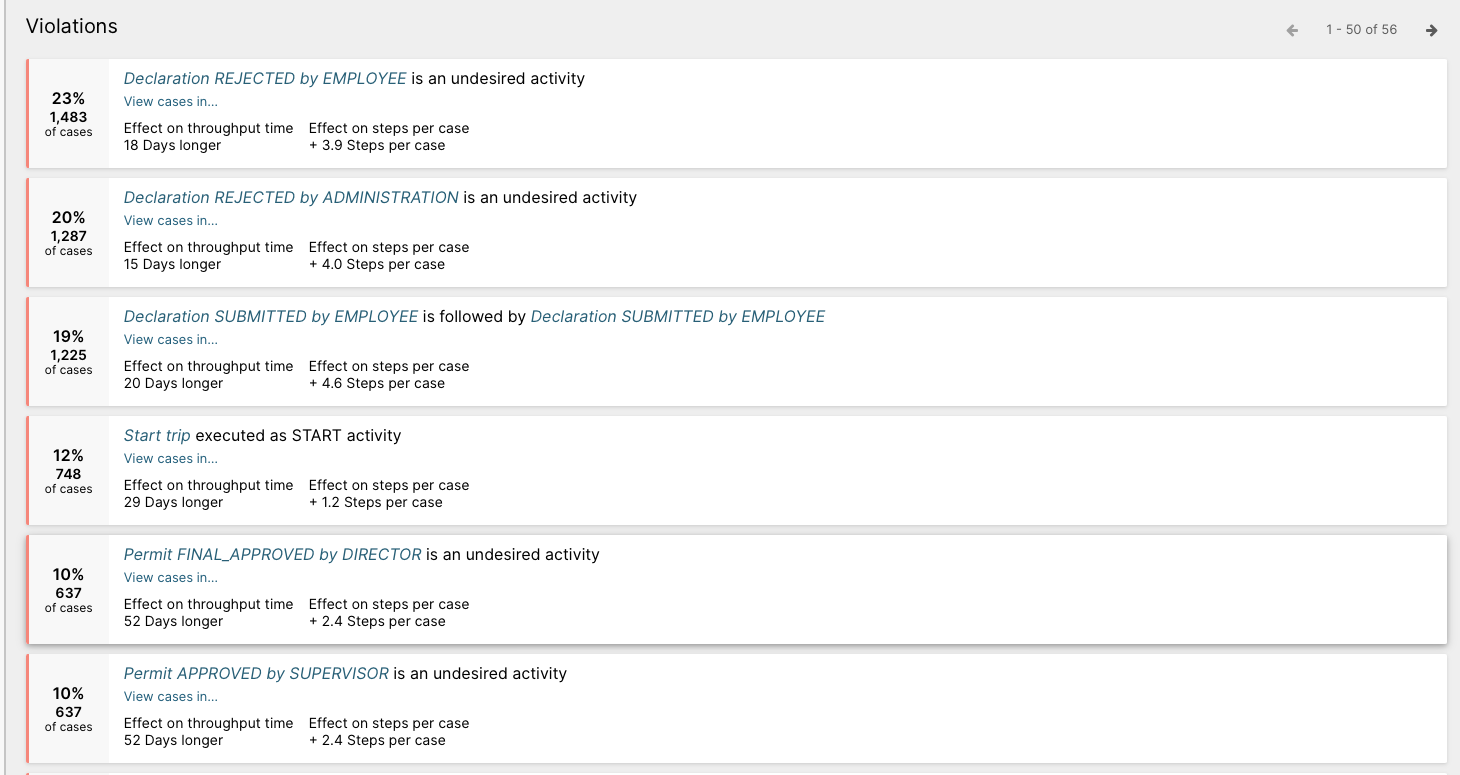
\includegraphics[width=\textwidth]{figures/celonis/int_violations.png}
		\caption{International}
	\end{subfigure}
	\caption{Häufigste Abweichungen vom Referenzmodell mit Effekt auf Durchlaufzeit und Schrittanzahl (Celonis \textit{Conformance})}
	\label{fig:violations}
\end{figure}

% ==================================================================
\subsection{Muster mangelnder Konformität}
\label{sec:nonconformance}

Conformance Checking gleicht das im Event-Log beobachtete Verhalten systematisch mit einem Prozessmodell ab \parencite{carmona_conformance_2018}. Eine zentrale methodische Erkenntnis dieser Untersuchung ist, dass die gemessene Konformitätsquote sowie ihre zeitliche Entwicklung unmittelbar von der Wahl und dem Abstraktionsgrad des zugrundeliegenden Referenzmodells abhängen. Um diesen Effekt nachzuweisen, wurde das Conformance Checking in Celonis zweistufig durchgeführt (\autoref{fig:conformance_comparison} sowie \autoref{tab:kpi_comparison}):

\begin{enumerate}[noitemsep]
    \item \textbf{Striktes Happy-Path-Modell (nur Variante 1):} Wird im Domestic-Log ausschließlich die häufigste Prozessvariante als Soll-Modell definiert (\autoref{fig:conf_model_strict}), beträgt die Gesamtkonformität exakt 44\,\% (4.618 Cases) (\autoref{fig:conf_hist_strict}). Der zeitliche Verlauf offenbart dabei ein extremes Muster: Von Januar bis Oktober 2017 liegt die Konformitätsquote bei $\approx 0\,\%$ und springt erst im Januar 2018 unvermittelt auf konstant 55--60\,\%.
    \item \textbf{Erweitertes Kernmodell (Top-3-Varianten mit XOR-Gateways):} Werden über exklusive Gateways (XOR) zusätzlich die Freigabe durch den \texttt{BUDGET OWNER} (Variante 2, 23\,\%) sowie das Überspringen der Administration (Variante 3, 13\,\%) als optionale Pfade zugelassen (\autoref{fig:conf_model_top3}), steigt die Gesamtkonformität auf 81\,\% (8.470 Cases). Gleichzeitig erhöht sich die Konformität im Jahr 2017 sprunghaft auf 50--75\,\% und erreicht ab Januar 2018 Werte zwischen 80\,\% und 90\,\% (\autoref{fig:conf_hist_top3}).
\end{enumerate}

Ein völlig analoges Bild zeigt sich im International-Log: Gegenüber dem strikten Happy-Path-Modell (21\,\% Gesamtkonformität, 1.369 Cases) liegt die Konformität bis einschließlich Dezember 2017 ebenfalls bei 0\,\% und steigt erst im erweiterten Modell (Top-3-Varianten mit XOR-Verzweigungen für Administration und Budget Owner) auf insgesamt 38\,\% (2.470 Cases; 20--35\,\% in 2017 vs.\ 40--47\,\% ab 2018; siehe \autoref{fig:conformance_comparison_int} im Anhang).

\begin{figure}[htbp]
    \centering
    % --- Obere Zeile: BPMN-Referenzmodelle ---
    \begin{subfigure}[t]{0.49\textwidth}
        \centering
        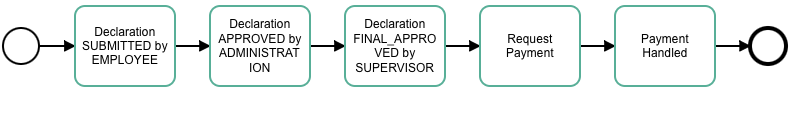
\includegraphics[width=\textwidth]{figures/celonis/dom_bpmn_v1.png}
        \caption{Striktes Happy-Path-Modell (nur Variante 1)}
        \label{fig:conf_model_strict}
    \end{subfigure}
    \hfill
    \begin{subfigure}[t]{0.49\textwidth}
        \centering
        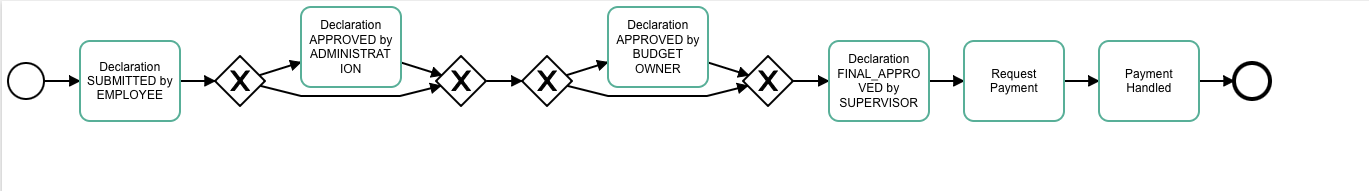
\includegraphics[width=\textwidth]{figures/celonis/dom_bpmn_top3.png}
        \caption{Erweitertes Kernmodell (Top-3-Varianten mit XOR)}
        \label{fig:conf_model_top3}
    \end{subfigure}

    \vspace{0.4cm}

    % --- Untere Zeile: Zugehörige Conformance-Verläufe ---
    \begin{subfigure}[t]{0.49\textwidth}
        \centering
        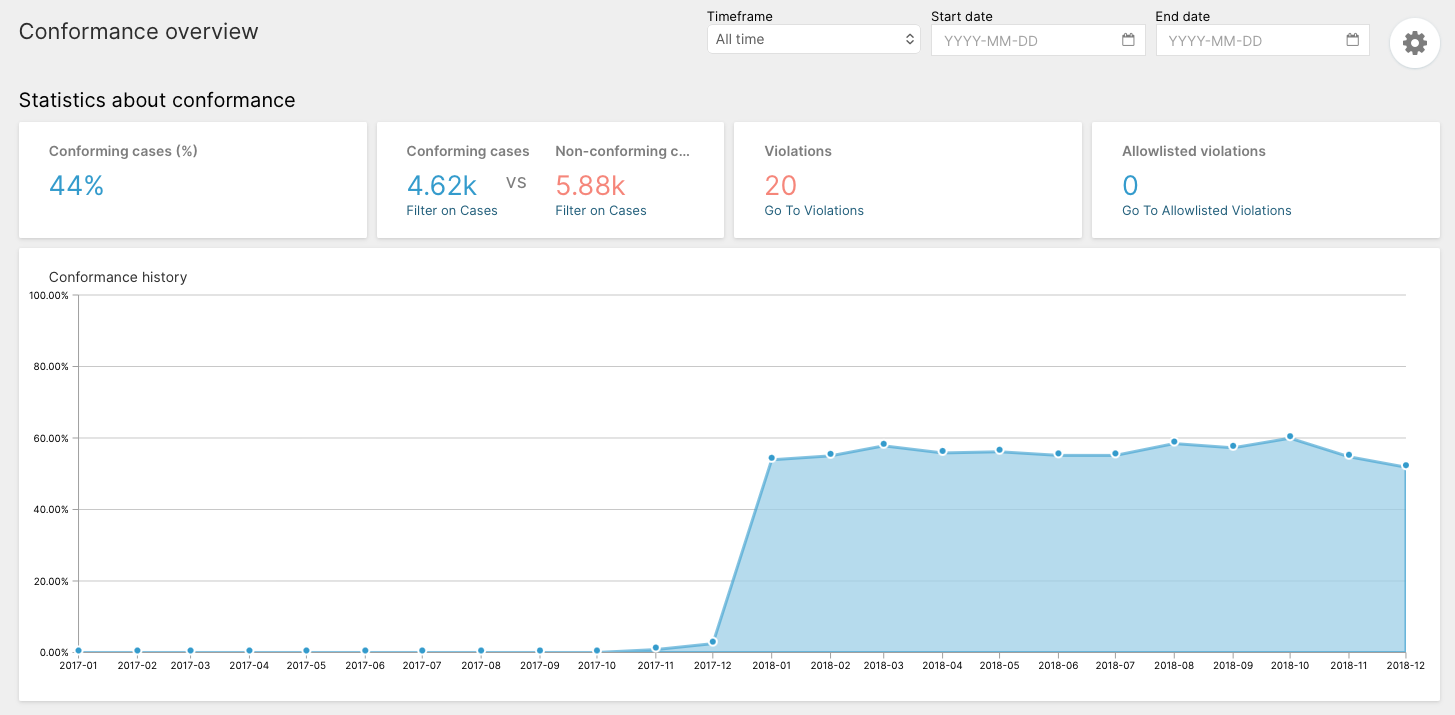
\includegraphics[width=\textwidth]{figures/celonis/dom_conf_v1.png}
        \caption{Konformitätsverlauf bei striktem Happy Path (44\,\%)}
        \label{fig:conf_hist_strict}
    \end{subfigure}
    \hfill
    \begin{subfigure}[t]{0.49\textwidth}
        \centering
        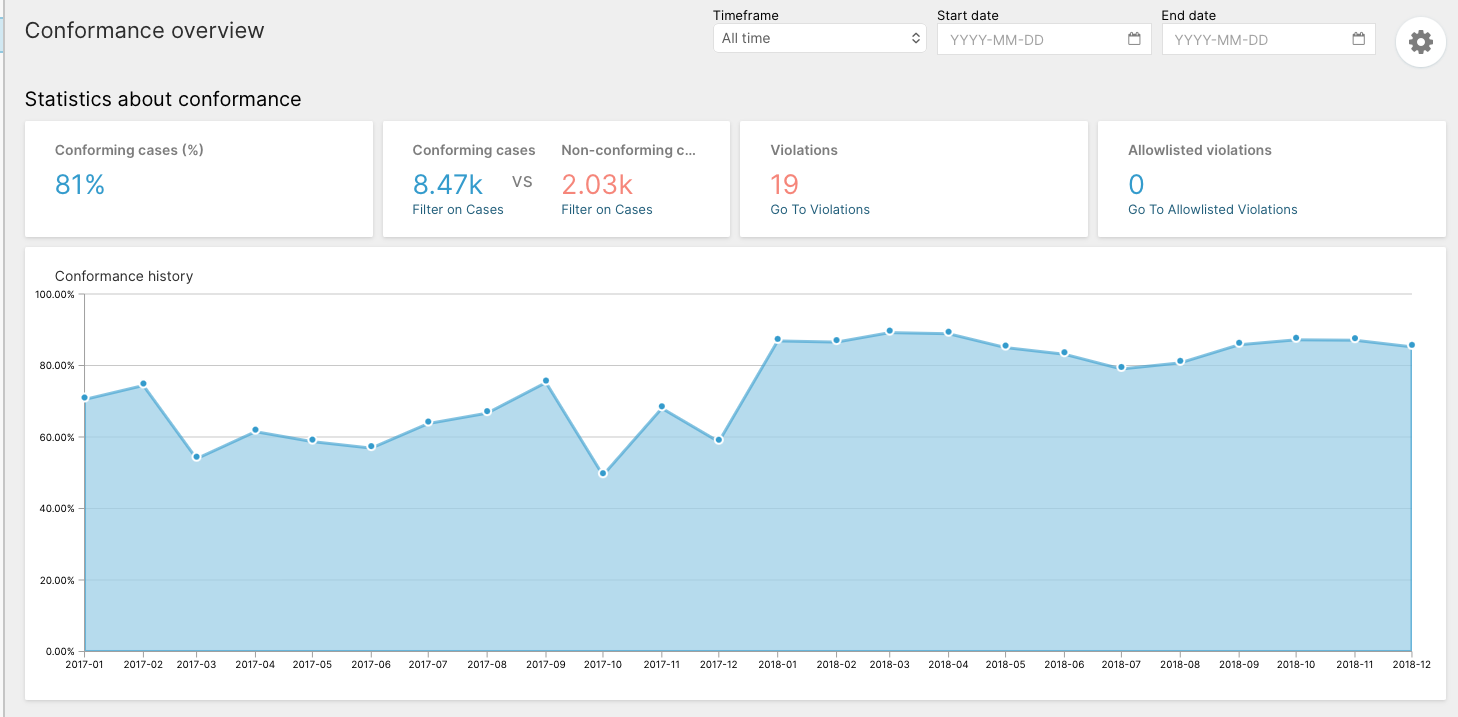
\includegraphics[width=\textwidth]{figures/celonis/dom_conf_top3.png}
        \caption{Konformitätsverlauf bei Top-3-Varianten (81\,\%)}
        \label{fig:conf_hist_top3}
    \end{subfigure}

    \caption{Einfluss des Referenzmodells auf die gemessene Konformität im Domestic-Log (links: nur Variante 1 mit $\approx 0\,\%$ Konformität in 2017; rechts: Top-3-Varianten inkl.\ Budget Owner)}
    \label{fig:conformance_comparison}
\end{figure}

\paragraph{Zeitlicher Verlauf und das Rollout-Artefakt 2018.}
Aus diesem Modellvergleich lassen sich zwei zentrale Schlüsse über die Prozesslandschaft der Universität ziehen. Erstens existierte der globale \enquote{Happy Path} (Variante 1) im Jahr 2017 in den beiden zuerst erfassten Pilotfakultäten faktisch nicht; dort durchliefen sämtliche Abrechnungen zwingend entweder einen \texttt{BUDGET OWNER}, einen \texttt{PRE\_APPROVER} oder übersprangen die Administration. Zweitens erklärt sich der markante Konformitätsanstieg zum Januar 2018 in beiden Logs nicht durch eine plötzliche operative Prozessverbesserung, sondern durch die Ausweitung der Datenerfassung auf die gesamte Universität \parencite{van_dongen_bpi_2020}. Da das Jahr 2018 rund viermal so viele Fälle umfasst wie das Pilotjahr 2017 (\autoref{tab:basisstatistik}), dominieren die neu angeschlossenen Fakultäten – in denen der schlanke Prozess ohne Budget Owner den Standard bildet – die Häufigkeitsverteilung des Gesamt-Logs. Ein datengetrieben aus den häufigsten Varianten generiertes Referenzmodell unterliegt somit einem Mengen-Bias zugunsten des Jahres 2018 und stuft abweichende Fakultätsprozesse aus 2017 systematisch häufiger als nicht konform ein.

\paragraph{Deskriptive vs.\ normative Modellgrenzen.}
Zugleich verdeutlicht das erweiterte Kernmodell (81\,\% bzw.\ 38\,\% Konformität) den Unterschied zwischen einem \emph{deskriptiven} (frequenzbasierten) und einem \emph{normativen} (regelgetriebenen) Referenzmodell: Ob eine Aktivität in Celonis als Regelverletzung (\enquote{undesired activity}) gewertet wird, hängt hier allein davon ab, ob sie in den ausgewählten Top-Varianten enthalten ist. Während die Freigabe durch den \texttt{BUDGET OWNER} (27--28\,\% der Cases) durch die Aufnahme der Varianten 2 und 3 als konform gilt, wird die fachlich vergleichbare Vorprüfung durch den \texttt{PRE\_APPROVER} (6\,\%, 666 Cases) als Verletzung gezählt (\autoref{fig:violations}), obwohl auch sie einen legitimen organisatorischen Prüfschritt darstellt. Die Allowlist von Celonis wurde bewusst nicht genutzt (0 allowlisted violations), um diese unverzerrten Rohwerte offenzulegen. Umgekehrt dürfte das automatisch generierte BPMN-Modell in Celonis aber auch nicht unkritisch auf weitere Varianten (z.\,B.\ Top-5) ausgeweitet werden: In diesem Fall würden auch Ablehnungsschleifen (\texttt{Declaration REJECTED by ADMINISTRATION} $\rightarrow$ \texttt{REJECTED by EMPLOYEE}) über ein XOR-Gateway als regulärer Modellpfad aufgenommen, wodurch echte Prozessfehler fälschlicherweise als \enquote{konform} eingestuft würden.

\paragraph{Zusammenfassung der Non-Conformance-Muster.}
Unter Berücksichtigung dieser Modellcharakteristik identifiziert Celonis im erweiterten Kernmodell 19 Verletzungstypen im Domestic- und 56 im International-Log. Nicht konforme Fälle dauern im Mittel 5,9 Tage (16,3 vs.\ 10,4\,d, Domestic) bzw.\ 27,8 Tage (97,1 vs.\ 69,3\,d, International) länger und erfordern durchschnittlich 1,3 bis 1,6 zusätzliche Prozessschritte (\autoref{tab:kpi_comparison}). Inhaltlich verdichten sich die Abweichungen auf vier zentrale Muster:

\begin{enumerate}[noitemsep]
    \item \textbf{Rework-Schleifen:} Ablehnungen mit anschließender Korrektur und Neueinreichung (\autoref{sec:rejections}) bilden in beiden Logs die häufigste und zeitintensivste Abweichung.
    \item \textbf{Umgehung der Vorab-Genehmigungspflicht:} 12\,\% der Auslandsreisen starten gänzlich ohne eingereichtes Permit; in weiteren Fällen wird die Genehmigung erst nach Reiseende eingeholt (\autoref{sec:unerwartet}).
    \item \textbf{Verzögerte Einreichung:} Deklarationen werden nach Reiseende erst mit erheblichem Verzug (Ø 13 Arbeitstage) eingereicht (\autoref{sec:bottlenecks}).
    \item \textbf{Zusätzliche Eskalations- und Prüfstufen:} Die Einbindung von \texttt{PRE\_APPROVER} und \texttt{DIRECTOR} verlängert die Durchlaufzeit signifikant (bis zu +52\,d) und wird vom frequenzbasierten Modell als Verletzung markiert, stellt fachlich jedoch meist einen regelkonformen Sonderpfad dar.
\end{enumerate}

	\section{Erweiterte Analysen und KPIs}
\label{sec:erweitert}

% Umfang: ca. 3 Seiten
% Assignment-Fragen 8-10:
%   8  What is missing to provide more detailed insights into the processes?
%   9  Where could supervised / unsupervised ML techniques help?
%   10 Can you think of useful KPIs for the processes?

\subsection{Fehlende Daten}
\label{sec:fehlende_daten}
Dass 2018 die Scope-Änderung von 2017 nicht dokumentiert wurde, ist ein Beispiel dafür, dass die Log-Daten nicht alle relevanten Informationen enthalten.
2018 wurde offenbar nicht nur die Datenerhebung erkennbar hochgeschraubt, indem weitere Fakultäten angebunden wurden, sondern auch der Prozess selbst verändert.
Mehrere ähnliche Prozesse im selben Log sorgen dafür, dass das Modell flexibler werden muss, um mehr abzudecken.
Anzunehmen ist, dass auch abseits vom Jahreswechsel zu 2018 weitere Änderungen im Prozess stattgefunden haben.
Auch verbleibt Unsicherheit darüber, ob alle Traces von vornherein aufgezeichnet oder ggf. nachträglich im Rahmen einer Art Migration nachgetragen wurden, um das Log zu vergrößern.
Prozessabläufe in International ohne Permit, falscher Permit id, mit identischer Reise und Payment sind ein Indiz dafür, dass hier Informationen ausblieben.
Wichtig ist auch, eine feste Liste gültiger Prozessabschlüsse zu haben. So sind nun mehrere Traces ohne vollständige Declaration-Bearbeitung enthalten, die nur ein Saved-Event enthalten.
Weiter ist die Rollenhistorie der Akteure nicht dokumentiert und unklar, wann welche Akteure organisatorisch eingeführt worden sind oder wie die Kompetenzen verteilt sind.
So sind die Bedeutungen des Budgets und den Limits nicht klar erkennbar.
Ebenfalls sind noch die Bedeutungen und Gründe der verschiedenen Ablehnungsoperationen unklar, um effektive Schlussfolgerungen zu treffen. \par
Bestätigt ist auch noch nicht, ob und wie Evententitäten (z.B. Declaration, Permit, Payment) wirklich miteinander verknüpft sind und auch so gelebt werden oder doch es sich nur um eine sprachliche Bündelung handelt ohne nähere Abläufe.
Mit der Ergänzung dieser Daten könnten je Zeitpunkt die wahren zugrundeliegenden Prozessvarianten identifiziert werden, was das Fitness und die Präzision unterstüzen würde und bestätigte Objektkontexte berücksichtigen kann.
% Eine kritische Reflexion darüber, welche Daten oder Attribute in den Logs fehlen.
% - keine Ablehnungsgründe
% - org:resource anonymisiert (nur STAFF MEMBER / SYSTEM) -> keine Social-Network-/Workload-Analyse
% - nur Abschluss-Events, keine Start-Events -> nur Warte-, keine Bearbeitungszeiten
% - keine Reisemerkmale (Ziel, Dauer, Kategorie)
% - keine Dokumentation der Scope-Änderung 2017 -> 2018


\subsection{Potenziale des maschinellen Lernens}
\label{sec:ml}

% Überwacht: Outcome-orientiertes Predictive Process Monitoring (Ablehnung ja/nein,
%   lange Durchlaufzeit) aus Präfix + Case-Attributen \parencite{teinemaa_outcome-oriented_2019}
% Unüberwacht: Anomalieerkennung \parencite{nolle_binet_2022}, Trace-Clustering
% Optional: Prototyp von Jesco (Python)

\todo{ML-Potenziale (Jesco)}

\subsection{Key Performance Indicators}
\label{sec:kpis}

% Definition + PQL-Formel + Werte Domestic/International \parencite{dumas_fundamentals_2018,vogelgesang_celonis_2022}
% Vorschläge: Median-Durchlaufzeit, First-Time-Right-Quote, Rework-Quote,
%             Permit-Compliance, Einreichungsverzug nach Reise, Zahlungsdauer
% Dashboard-Screenshots nach figures/celonis/

\todo{KPIs mit PQL (Eziz)}

	%\section{Tool-Vergleich: Celonis vs. Python}
\label{sec:toolvergleich}

% Umfang: 1-2 Seiten
% Assignment: "Pick two out of three ... Compare the results!"
% - Gegenüberstellung der beiden gewählten Werkzeuge (Vergleichstabelle):
%   Bedienung, Exploration/Visualisierung, Discovery, Conformance (Happy Path vs.
%   Alignments auf normativem Modell), Reproduzierbarkeit, ML-Erweiterbarkeit, Kosten.
% - Stärken Celonis (schnelle visuelle Exploration, Dashboarding, PQL) vs.
%   Python/PM4Py (Flexibilität, spezifische Algorithmen) \parencite{berti_process_2019,vogelgesang_celonis_2022}
% - Ergebnisvergleich: Abweichungen bei Varianten, Durchlaufzeiten, Konformitätsquote?
%   * Durchlaufzeit International: Celonis zeigt 86 d (alle Cases, Throughput Times),
%     75 d (ohne Extremwerte, Process Overview) und 66 d (Happy Path). Ein mean() in
%     Python ergibt ~86 d -> Beispiel dafür, dass Standard-KPIs in BI-Tools still
%     trimmen und von Rohdaten-Berechnungen abweichen (vgl. Abschnitt 3.1).
%   * Konformität: Celonis prüft gegen ein aus den Top-Varianten generiertes Modell
%     (81 % / 38 %), PM4Py gegen normatives Modell (Alignments) -> Werte nicht 1:1 vergleichbar.
%   * Datenqualität: 134 Domestic-Cases mit nur "Declaration SAVED" (0 d Durchlaufzeit)
%     -> beeinflussen Mittelwerte je nach Filterung in beiden Tools unterschiedlich.

\todo{Tool-Vergleich (gemeinsam)}

	\section{Tool-Vergleich und Fazit}
\label{sec:fazit}

\subsection{Tool-Vergleich: Celonis vs.\ Python (PM4Py)}
\label{sec:toolvergleich}

Die parallele Untersuchung mit der kommerziellen Plattform Celonis und der Open-Source-Bibliothek PM4Py zeigt, dass sich beide Werkzeuge komplementär ergänzen, in der Datenverarbeitung und bei einzelnen Kennzahlen jedoch methodisch bedingte Abweichungen aufweisen (\autoref{tab:toolvergleich}).

\begin{table}[htbp]
\centering
\caption{Systematischer Vergleich von Celonis und Python (PM4Py) im Analyseprozess}
\label{tab:toolvergleich}
\footnotesize
\renewcommand{\arraystretch}{1.15}
\begin{tabularx}{\textwidth}{@{}p{2.9cm} X X@{}}
\toprule
\textbf{Dimension} & \textbf{Celonis (Process Analytics \& PQL)} & \textbf{Python (PM4Py)} \\
\midrule
\textbf{Datenimport \& Attribute} &
Direkter XES-Import erzeugt nur eine Aktivitätstabelle; Trace-Attribute (\texttt{Amount}, \texttt{Permit ID}) fehlen ohne vorherige CSV-Konvertierung. &
Voller Zugriff auf alle Trace- und Event-Attribute; deckt 448 Dummy-Permits (\texttt{travel permit 423}) und 3.078 redundante Event-IDs auf. \\
\textbf{Exploration \& Vorverarbeitung} &
Sehr schnelle, interaktive Filterung über Varianten, Zeiträume und Einzelfälle (\textit{Case Explorer}); PQL erlaubt flexible KPI-Dashboards. &
Hohe algorithmische Freiheit: Text-Clustering der 37 Eventnamen (Exact Cover / Algorithmus X), Entfernen der Trip-Events und Zeitsplits. \\
\textbf{Process Discovery \& Conformance} &
Frequenzbasierter Process Explorer und BPMN-Abgleich (Variante 1 vs.\ Top-3 mit XOR); visualisiert den Strukturbruch 2018 unmittelbar. &
Systematisches Benchmarking vieler Miner (Heuristic, Inductive, ILP); exakte Fitness-, Precision- und F1-Berechnung (Anstieg von 0,902 auf 0,961). \\
\textbf{Ergebnisvergleich (Kennzahlen)} &
Varianten: 100 (Dom.) / 756 (Int.).\newline
Ø Durchlaufzeit Int.: weist je nach View 66\,d (Happy Path), 75\,d (getrimmt) oder 86\,d (alle Cases) aus. &
Varianten: 99 (Dom.) / 753 (Int.) (Tie-Breaking bei gleichen Zeitstempeln).\newline
Ø Durchlaufzeit Int.: 86\,d auf Rohdaten. \\
\bottomrule
\end{tabularx}
\end{table}

\subsection{Fazit und Limitationen}
\label{sec:zusammenfassung}
Trotz prozessualer Veränderungen im Zeitverlauf, konnten bereits mit den Rohdaten in Celonis und in Python mögliche Prozessabläufe identifiziert werden, die zu einer starken Abdeckung der Gesamtlogs führen.
Mit F1-Scores von über 0,9 konnte konsequent bestätigt werden, dass die Prozessmodelle die beobachtbaren Event-Logs abbildeten.
Mithilfe von Textanalyse und Exact-Cover-Clustering konnten zudem mögliche Objektzentrierungen und Aktivitäten-Clustering stattfinden, was die Interpretation stütze.\par
Es lässt sich festhalten, dass für inländische (Domestic) Reisen eine Reisekostenabrechnung (Declaration) vorangeht, um die Bezahlung nach einem mehrstufigen Genehmigungsprozess freizugeben.
Für internationale (International) Reisen wird hingegen auch ein Reiseantragsgenehmigungsprozess (Permit) vorausgesetzt, um die Reisekostenabrechnung loszutreten. Zusätzlich werden im International-Log auch Reminder verschickt im Gesamtprozess und auch die Reisedaten (Trip) erfasst.
Auffällig ist, dass in dem internationalen Log identische Events mehrfach vorkommen und "wiederverwendet" werden.
Auch gibt es Fälle, in denen in den Trace-Metadaten -- welche belastbar ausführlicher sind als beim Domestic-Log -- Permit-Metadaten anders befüllt werden und in dieser Abweichung ein Zusammenhang mit International-Traces ohne Reisegenehmigung (Permit) vorliegt.
In diesen Fällen konnte eine Reisekostenabrechnung (Declaration) ohne Reisegenehmigung (Permit) stattfinden, was auf eine mögliche Prozessabweichung hindeutet und zunächst nicht als konform wirkt in Rücksicht auf den geringen Trace-Anteil.
\par
Cash-Flows (Payment) bedingen im Allgemeinen den Abschluss des Genehmigungsprozesses komplett. In beiden Logs finden sich dafür aber auch Gegenbeispiele, bei denen das Payment durchgeführt wurde, bevor eine volle Genehmigung vorlag.
Im Log waren zudem auch nicht nur konforme positiv abgeschlossene Fälle enthalten, sondern auch 1301 (Domestic) bzw. 1755 (International) abgelehnte Fälle, bei denen im Log keine weitere Bearbeitung erfolgte.
Bei diesen Traces ist von einer finalen Ablehnung auszugehen. Insgesamt konnte der Grundprozess annähernd präzise abgebildet werden, wobei festgestellt wird, dass weitere Metainformationen zur Prozesshistorie und Organisationen unterstützen würden.



% ###############################################################

	\newpage
	\pagenumbering{Roman} % Römische Seitenzahlen aktivieren
	\setcounter{page}{\theromanBeginningEnd} % Römische Seitenzahlen fortsetzen
	\setcounter{secnumdepth}{0} % Nummerierung der Überschriften entfernt

% Quellenverzeichnis
	\setcounter{secnumdepth}{3} % Überschriften wieder numerieren (Für den Anhang)

	% Uncomment to use APA
	%\bibliography{Quellenverzeichnis}

	% Uncomment to use IEEE
	\printbibliography % Quellenverzeichnis drucken

	\newpage

% ANHANG
	\appendix
\phantomsection
\addcontentsline{toc}{section}{Anhang}
\section*{Anhang}
\label{sec:anhang}
 % Anhang einfügen
	\clearpage % Floats des Anhangs abschließen, sonst rutschen sie in die Erklärung

	\pagenumbering{gobble} % Seitenzahlen entfernen
% top right corner
\thispagestyle{fancy}
\fancyhf{}
\rhead{
\includegraphics[width=0.4\textwidth]{resources/Logo.png}}

\section*{Eigenständigkeitserklärung}
Mit unserer Unterschrift versichern wir, dass wir die hier vorliegende Arbeit selbständig, ohne
fremde Hilfe und nur mit den angegebenen Hilfsmitteln verfasst haben und unsere Angaben zu
den verwendeten Quellen der Wahrheit entsprechen und vollständig sind. Alle Quellen, aus
denen wir wörtlich oder sinngemäß übernommen haben, haben wir als solche gekennzeichnet.

Darüber hinaus versichern wir, dass wir sämtliche Teile der vorliegenden Arbeit, die unter
Zuhilfenahme künstlicher Intelligenz (KI) generiert wurden, als solche gekennzeichnet haben und
deren Entstehung in einer beigefügten Prozessdokumentation nachgewiesen haben.

Wir haben zur Kenntnis genommen, dass zuwiderlaufendes Verhalten als Täuschungsversuch
gewertet wird und zu den in der geltenden Prüfungsverfahrensordnung genannten
Konsequenzen führen wird.
\newline
\newline
    Hannover, den 18.10.2026 \hfill
\includegraphics[width=4cm,valign=c]{resources/Unterschrift_homb} Jesco Cedric Homberg
	\vspace{8mm}

	Nürnberg, den 18.10.2026 \hfill
\includegraphics[width=4cm,valign=c]{resources/Unterschift_eziz.png} \hfill Eziz Muhammedkulyyev
	\vspace{8mm}
 % Eigenständigkeitserklärung einfügen
	\newpage
	\begin{landscape}
\definecolor{color_30879}{rgb}{0,0.12549,0.376471}
\pagenumbering{gobble} % Seitenzahlen entfernen
    % top right corner
    \thispagestyle{fancy}
    \fancyhf{}
    \rhead{
\includegraphics[width=0.4\textwidth]{resources/Logo.png}}

\section*{Prozessdokumentation}
\textbf{Für die Nutzung von Künstlicher Intelligenz (KI) in wissenschafftlichen Arbeiten}
\vspace{3mm}

\noindent\textbf{\large Eziz Muhammedkulyyev}
\vspace{3mm}

\begin{longtable}{|p{6.5cm}|p{5cm}|p{8cm}|p{4cm}|}
\hline
\rowcolor{color_30879}
\textbf{\textcolor{white}{Anfrage an folgende KI (inkl. Abrufdatum)}} &
\textbf{\textcolor{white}{Grund für die Verwendung der KI}} &
\textbf{\textcolor{white}{Bewertung der Qualität des KI-Outputs}} &
\textbf{\textcolor{white}{Verwendete Software und Versionsnummer}} \\
\hline
\endhead
\hline
„Warum werden beim direkten XES-Import von \texttt{DomesticDeclarations.xes} und \texttt{InternationalDeclarations.xes} in Celonis keine Case-Attribute wie \texttt{Amount} oder \texttt{Permit ID} als eigene Case-Tabelle angelegt, und wie lässt sich das in Celonis prüfen?“ (16.10.2026) &
Klärung technischer Fragen zu Celonis und zu den Einschränkungen des nativen XES-Imports (Kapitel 4.3) &
Die Erklärung, dass der Standard-XES-Import in Celonis nur die Event-Ebene in eine Aktivitätstabelle übernimmt und Trace-Attribute abflacht, war zutreffend. Ich habe dies im Celonis-Datenmodell überprüft und anhand der offiziellen Celonis-Dokumentation sowie des Community-Eintrags (Buijs, 2019) verifiziert. &
Google Gemini / Antigravity \\
\hline
„Erstelle PQL-Formeln in Celonis für die Durchlaufzeit zwischen \texttt{Declaration SUBMITTED by EMPLOYEE} und \texttt{Payment Handled}, für Mehrfacheinreichungen sowie Filter für abgelehnte Cases.“ (mehrfach, 15.--17.10.2026) &
Teilweise Generierung und Fehlersuche bei PQL-Abfragen für eigene Analyse-Views (\textit{TPT Analysis}, \textit{Rejections Dashboard}) und KPIs (Kapitel 4 und 5.3) &
Die vorgeschlagenen PQL-Ausdrücke (u.\,a.\ mit \texttt{CALC\_THROUGHPUT}, \texttt{FIRST\_OCCURRENCE} und \texttt{PU\_COUNT}) waren als Vorlage hilfreich, mussten jedoch teilweise an die exakten Spaltennamen im Celonis-Datenmodell angepasst werden. Alle Abfragen habe ich in Celonis selbst ausgeführt und die Ergebnisse an Einzelfällen geprüft. &
Google Gemini / Antigravity \\
\hline
„Wie unterscheiden sich die ausgewiesenen Durchlaufzeiten in den Celonis-Standard-Views (\textit{Process Overview} vs.\ \textit{Throughput Times}) und wie verhält sich der Conformance-Checker beim Erweitern des Referenzmodells auf die Top-3-Varianten?“ (16.10.2026) &
Rückfragen zur Funktionsweise von Celonis bei der Kennzahlenaggregation und beim Conformance Checking (Kapitel 4.1 und 4.5) &
Die Hinweise zur internen Ausreißer-Filterung im \textit{Process Overview} und zur Generierung von XOR-Gateways im Conformance-Checker waren nachvollziehbar. Die fachliche Interpretation (insbesondere zum Rollout-Effekt 2018 und zur Rolle \texttt{REJECTED by EMPLOYEE}) habe ich selbst anhand der Dashboards und des \textit{Case Explorers} erarbeitet. &
Google Gemini / Antigravity \\
\hline
„Formuliere aus meinen Celonis-Kennzahlen, Screenshots und Stichpunkten zu Durchlaufzeiten, Bottlenecks, Ablehnungen, Conformance und KPIs einen wissenschaftlich strukturierten LaTeX-Text für Kapitel 1, 4 und 5.3.“ (mehrfach, 16.--18.10.2026) &
Textgenerierung und sprachliche Ausformulierung in LaTeX auf Basis eigener Analyseergebnisse und Notizen &
Die generierten Textabschnitte setzten meine vorgegebenen Kennzahlen, Beobachtungen und Gliederungspunkte sprachlich sauber in LaTeX um. Sämtliche Zahlenwerte, Aussagen, Tabellen und Literaturverweise wurden von mir kritisch gegengelesen, teilweise umformuliert und mit meinen Celonis-Auswertungen abgeglichen. &
Google Antigravity / Gemini \\
\hline
\end{longtable}

\newpage

\noindent\textbf{\large Jesco Cedric Homberg}
\vspace{3mm}

\begin{longtable}{|p{6.5cm}|p{5cm}|p{8cm}|p{4cm}|}
\hline
\rowcolor{color_30879}
\textbf{\textcolor{white}{Anfrage an folgende KI}} &
\textbf{\textcolor{white}{Grund für die Verwendung der KI}} &
\textbf{\textcolor{white}{Bewertung der Qualität des KI-Outputs}} &
\textbf{\textcolor{white}{Verwendete Software und Versionsnummer}} \\
\hline
\endhead
\hline
Zeilenweise Code-Vervollständigung während des Schreibens in der IDE (laufend) &
Beschleunigung wiederkehrender Schreibarbeit im Code &
Vorschläge ohne inhaltliche Tragweite. Jede Übernahme erfolgte bewusst und wurde beim Ausführen der Notebooks mitgeprüft. &
GitHub Copilot (Code-Completion) in PyCharm \\
\hline
Erklärung von Funktionalitäten von Pandas und PM4Py (laufend) &
Tiefenwissenslücken ergänzen &
Vorschläge ohne inhaltliche Tragweite. Es ging um Übersicht und Möglichkeiten, um zu prüfen, was nachgebaut werden muss und was bereits besteht. &
GitHub Copilot (Code-Completion) in PyCharm \\
\hline
Umsetzung eigener Entwürfe und Ablaufskizzen in ausführbaren Python-Code (laufend) &
Werkzeug zur Code-Generierung anhand des eigenen Entwurfs, da das eigene Python-Wissen breit, aber nicht in der nötigen Tiefe vorhanden ist &
Aufbau, Reihenfolge und inhaltliche Festlegungen stammen von mir, die KI hat sie in Code übersetzt. Vorschläge wurden ausnahmslos als lokaler Git-Diff gesichtet und erst nach eigener Prüfung übernommen. &
Claude (Anthropic), Opus 4.8 (GitHub Copilot, Max/1M) \\
\hline
Umsetzung eigener Entwürfe und Ablaufskizzen in ausführbaren Python-Code (Bsp. 1) &
Funktionsgenerierung &
Prompt: Bau mir bitte in dieses Notebook einen simplen Parser für die XES-Dateien unter resources (objektorientiertes Ziel). Cool wäre das in einer SQLite-Datenbank direkt zu speichern, damit ich direkt die strukturiert untersuchen kann zbd das nicht mehrfach machen muss. Ich glaube Events haben immer die gleichen 5 Felder, aber Trace scheint wohl teilweise auch mehr zu haben. Vielleicht macht da dann auch Sinn, die Nicht-Standardfelder in einer Map in einer Spalte AdditionalInfos oder sowas zu hinterlegen. Ein Informationsverlust darf nciht geschehen bei der Transformation zur DB &
Claude (Anthropic), Haiku 4.5 03.10.26 // 6.8 Credits (GitHub Copilot, Max/1M) \\
\hline
Umsetzung eigener Entwürfe und Ablaufskizzen in ausführbaren Python-Code (Bsp. 2) &
Funktionsgenerierung &
Prompt: Die Reihenfolge der members ist eigentlich egal: Ich möchte gerne eine Funktion schreiben, die für eine membersliste folgendes macht: Schablonartig übereinander legen und schauen, ob es Übereinstimmungen gibt. Erst basierend auf der Reihenfolge, aber unberücksichtigt eventuell zusätzlicher Wörter zwischen den Wörtern. Das sollte absichern, dass alle "Declaration xy by abc" gefunden werden mit einem Matcher "Declaration % by %" - Unübereinstimmungen sollen mit % gekennzeichnet werden. Für die beiden Payment-Actions kommt dann vermutlich "%Payment%" raus. Egal, kein Overfitting:
Ich glaube, dafür reicht entweder ein Textmatcher, aaaber es fühlt sich für mich auch noch Process Mining vom Vorgehen an, wo Ähnlichkeiten zweier Logs untersucht werden - vielleicht ist deswegen auch pm4py eine gute Möglichkeit. &
Claude (Anthropic), Opus 5.5 07.10.26 // 6.8 Credits (GitHub Copilot, Max/1M) \\
\hline
Syntaxhilfe und Styling von Diagrammen und technischer Projektstruktur &
Als Werkzeug zur Lösung von Syntaxproblemen, Inkonsistenzen in meinen Befehlen, aufgetretenden Refactoring-Problemen oder das Anpassen der Ausgabe-Styles von BPMN-Diagrammen oder Tabellen. Außerdem als Hilfe bei Problemen in der Programmumgebung. &
Aufbau, Reihenfolge und inhaltliche Festlegungen stammen von mir, die KI hat sie in Code übersetzt. Vorschläge wurden ausnahmslos als lokaler Git-Diff gesichtet und erst nach eigener Prüfung übernommen. &
Claude (Anthropic), Opus 4.8 (GitHub Copilot, Max/1M) \\
\hline
Umbenennung und Refaktorisierung der Jupyter-Notebooks &
Erhöhung der Übersicht und Vereinheitlichung der Projektstruktur durch Auslagerung in extra Funktionspackage &
Rein organisatorische Änderung, das Ergebnis habe ich gegen die Notebook-Reihenfolge geprüft. Ohne Einfluss auf den Inhalt der Arbeit. &
Claude (Anthropic), Opus 4.8 (GitHub Copilot, Max/1M) \\
\hline
\end{longtable}
\end{landscape}
 % KI-Erklärung einfü

\end{document}
